\section{Detector Systematic Effects}
\label{sec:detsys}

The detector related systematic uncertainty is the smallest source of systematic uncertainty in the absolute water cross section measurement. Also, there are a few corrections in detector modeling and simulation that must be applied to the cross section calculation. The sources of detector systematic uncertainty and correction are: 

\begin{enumerate}
\item P0D tracking and matching efficiency
\item Hit Reconstruction efficiency
\item Neutral back scattering
\item Fiducial volume
\item Sand muon background rate
\item Out of fiducial volume background
\item Event pile-up rate
\item Track timing
\item Cosmic background
\item TPC1 tracking efficiency
\item Charge mis-ID rate
\end{enumerate}

In the following sections we describe the evaluation of these uncertainty sources in great detail. We first evaluate the systematic uncertainties and present the results as an error on the ratio of total selected events in data to the total selected events in MC. The errors on the data/MC ratio are summarized in Table \ref{tab:syssum} following the discussion of the error calculation methodologies. With the exception of the TPC1 tracking efficiency and the charge mis-ID rate, all other work in this Section is entirely ours. The TPC1 tracking efficiency and the base charge mis-ID rates per TPC were provided to us by the Tracker group. Our contribution lies in propagating this information to an uncertainty on the absolute water cross section. 

In a subsequent section, we develop a formalism for propagation of data/MC ratio uncertainties to cross section measurement uncertainties. We also describe how we correct the cross section result for inaccuracies in the detector modeling and background simulation. Finally, the developed formalism is used in conjunction with the results from this section to yield the new central value and the detector systematic uncertainties of the absolute $\nu_\mu$ CC inclusive cross section on water.

\subsection{Track Matching Efficiency Uncertainty}
\label{sec:matchingsyst}

The efficiency of reconstruction, and the differences between Monte Carlo and data efficiencies, are the first source of systematic uncertainty studied for the CC inclusive selection. There are several steps involved in reconstructing the final candidate muon track as described in previous sections. In this section, we use a `FGD Cosmic' sample to  investigate the reconstruction and matching efficiencies of our analysis. Cosmics provide a sample independent of the physics we are probing, and are an excellent unbiased sample to use to evaluate the efficiency systematic. However, as Cosmics do not have the same bunched timing structure as our beam events, we also used as independent sample of sand muons to cross check our results. Sand muons are generated by beam neutrinos interacting with material outside the off-axis near detector and have the same timing as the beam events. The sand muon study is not shown, but efficiencies extracted from cosmics and sand muons agree well. Finally, we also performed a hand-scan of beam events in reconstruction files to identify and quantify any reconstruction issues missed with the FGD cosmics and sand muon samples.

We use a simple method to examine the efficiency of our matching algorithm for tracks that deposit energy in the P0D, enter the Tracker and are reconstructed by the Tracker reconstruction software. We simultaneously determine how often P0D reconstruction successfully fits a track and how often we succesfully match this track with a Tracker reconstructed track. First, we pre-select a sample of quality tracks reconstructed in TPC1 that point squarely into the 
P0D. We then attempt to pair each of these tracks to a P0D reconstructed track. The ratio of the number of matched pairs found to the number of quality TPC1 tracks yields the ``matching efficiency". Though this estimate is not necessarily the absolute efficiency, given that MC simulates data well to first order, the observed difference between the MC efficiency and the data efficiency gives us the systematic due to reconstruction and matching.

This definition folds in the P0D's intrinsic, lower level reconstruction efficiencies (i.e. hit finding, P0D-only tracking, etc.) as well as matching and recombination efficiencies from the matching algorithm. However, as we use reconstructed tracks in the ND280 Tracker as a baseline, we do not account for the Tracker tracking efficiency with this strategy. We determine the systematic uncertainty from the Tracker efficiency separately in a later section.

\subsubsection{Cosmics Sample}
\label{sec:CosmicsEfficiency}

Using the `FGD Cosmics' sample, we extract the matching efficiency as defined above. The following determine the denominator and numerator. Note that for the numerator of the efficiency, the cuts closely mimic those used in Section \ref{sec:selection} to select muon candidates. Also, the pre-selection cuts are slightly different between the Cosmics sample as opposed to the Sand Muon sample. The necessity for this difference is discussed later.

Pre-Selection Cuts (Denominator):

\begin{enumerate}
\item There must be a Tracker reconstructed track in the event
\item The Tracker track must be reconstructed as beginning at the upstream face of the first TPC (Z \(<\) -750 mm)
\item The TPC must measure a momentum of at least 250 MeV
\item Project the Tracker track linearly backwards into the P0D. The projection is made to the Z = -1100 mm plane, and then just the XY fiducial cut is applied to the projected point.
\item The Tracker track has \(>\) 18 reconstruction nodes
\item The Tracker track has a `corrected time' stamp between -4800ns and -4400ns. The time correction allows us to find the tracker time in relation to the P0D electronics. The time cut is placed 80ns from the edge of the 480ns-wide P0D integration window. This is the window where the P0D electronics are capable of properly reconstructing hits.
%\item There are at least 3 `good P0D hits'. A `good hit' is defined as a 7 p.e. or greater P0D hit which is found within a certain region of the P0D and with a certain time. The region we search is a cone with opening angle of 30 degrees and length of 250mm. The time is required to be 80ns from the edge of the P0D integration window. We make this cut to assure that no noise hits or hits with invalid timing due to known electronics design, are contaminating our pre-selection.
\end{enumerate}

Matching Cuts (Numerator):
\begin{enumerate}
\item All pre-selection cuts are made as above
\item P0D Vertex must be reconstructed by TP0DPairwiseVertexPID algorithm, proprietary reconstruction algorithm, and the track must be a constituent of this vertex
\item P0D Track must be exiting as defined by the last node having a Z position $>$ -1016 mm
\item P0D Track must be 3D as defined by cutting on track position variance
\item Evaluate $\Delta R$, $\Delta \sin \theta$  and $\Delta T$ between the p0d track projection and tracker track as before. Apply the following cuts: $\Delta R$ \(<\) 86mm, $\Delta \sin \theta$ \(<\) .76, $\Delta T$ \(<\) 100~ns.
\end{enumerate}

The number of tracks passing the numerator cuts divided by the number passing the denominator cuts yields the efficiency. Figures \ref{fig:eff_dR} and \ref{fig:eff_dSdT} show the matching parameter distributions for $\Delta R$, $\Delta X$, $\Delta Y$, $\sin \Delta \theta$ and $\Delta T$. 
The $\Delta Y$ distribution does not agree very well and causes some disagreement in the $\Delta R$ distribution as well. This discrepancy has been isolated to a difference between forward going and backwards going cosmics tracks as determined by the Tracker reconstruction. Figure \ref{fig:dY} shows the $\Delta Y$ residuals separated by forward and backwards going tracks for FGD cosmics in data and MC. Note that in MC, the two different directions have a small shift in the central value of the residual. However, in data, the shift is much greater. We have fit gaussians to all of the residuals and the results are shown in Table \ref{tab:FitdY}. The root cause of this effect is a difference in the geometry used for reconstruction and the geometry of the `as built' detector. Finally, note that since the $\Delta R$ agreement between data and MC for the Cosmics sample is actually worse than the beam events, the evaluated uncertainty should be conservative. 
Similarly, though the timing distribution does not agree as well as the others, the timing cut is large enough to account for the overall shift. 

\clearpage
\afterpage{
\begin{landscape}
\begin{figure}[h]
\centering
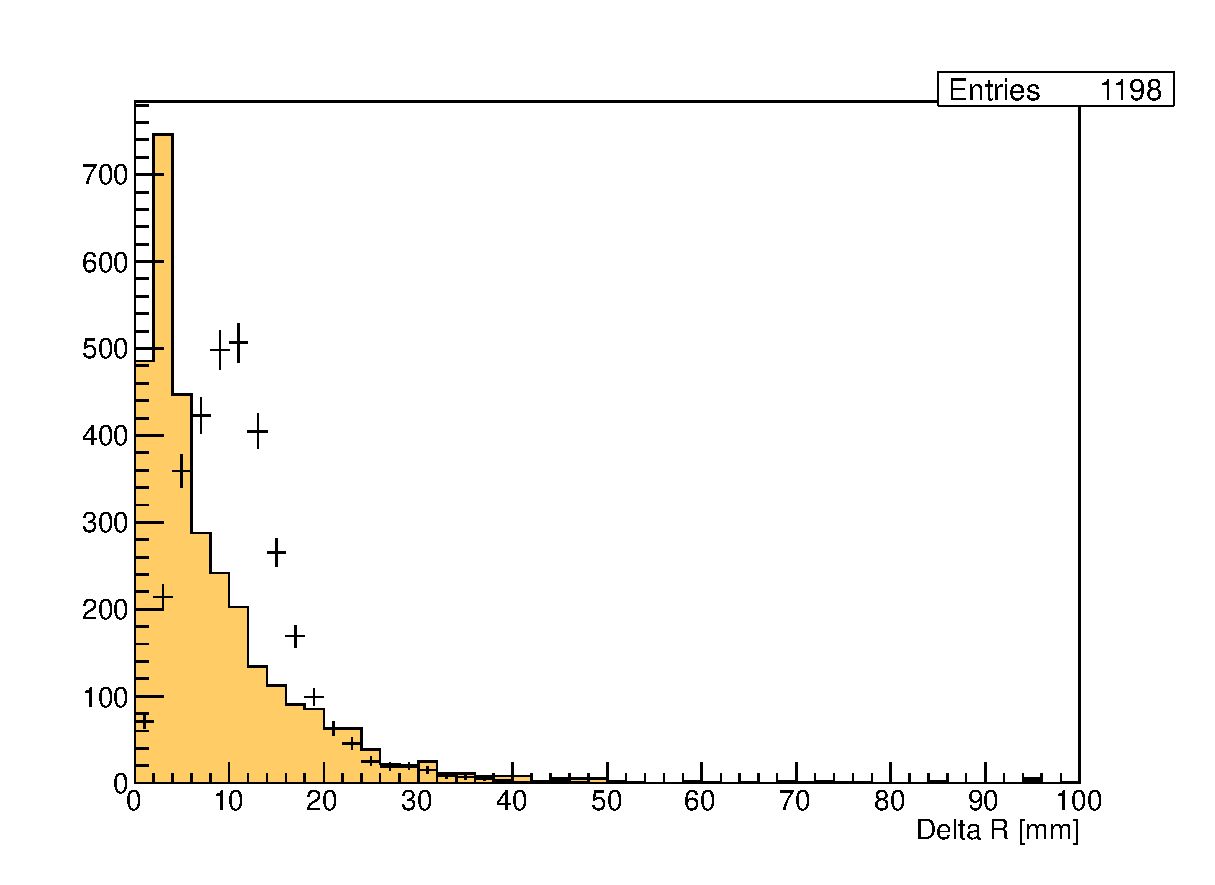
\includegraphics[width=3.25in]{Figures/Systematics/MatchingEfficiency/dRcosmics.eps}
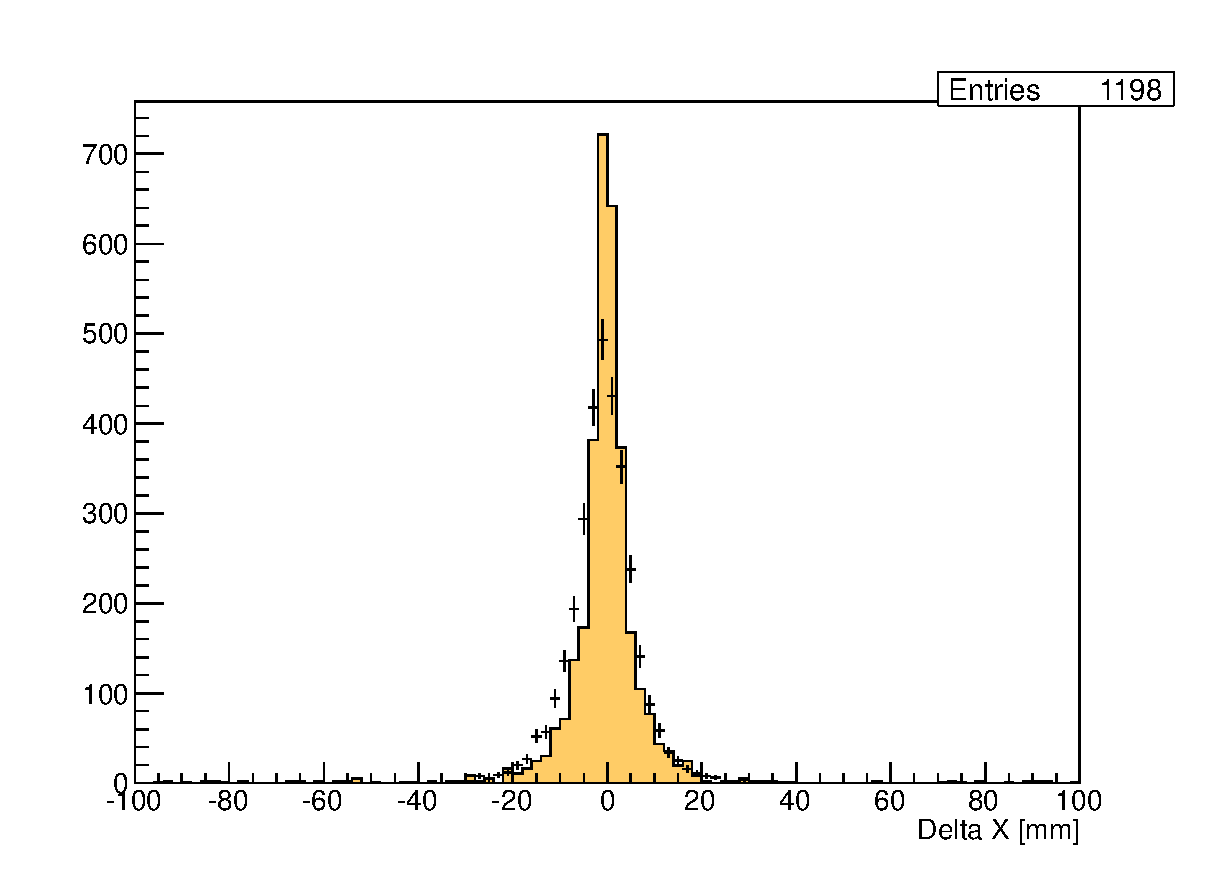
\includegraphics[width=3.25in]{Figures/Systematics/MatchingEfficiency/dXcosmics.eps}
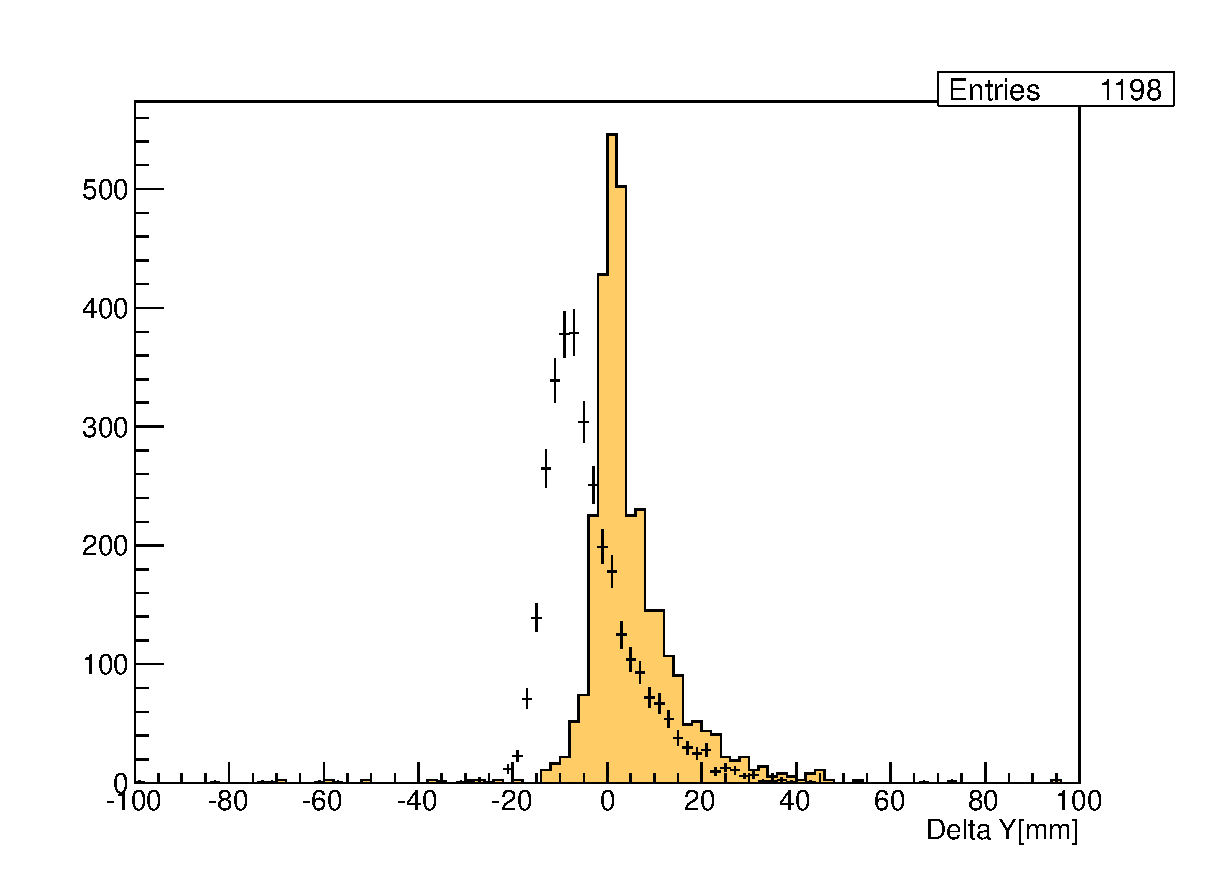
\includegraphics[width=3.25in]{Figures/Systematics/MatchingEfficiency/dYcosmics.eps} 
\caption{
Matching Parameters $\Delta$ R, $\Delta$ X, and $\Delta$ Y for cosmics. The matching cut is applied only on $\Delta$ R. Black dots with error bars denote data while the orange fill is MC. We note that the difference in shape in $\Delta$ R distributions is due to a shape difference in $\Delta$ Y between data and MC.
}
\label{fig:eff_dR}
\end{figure}

\begin{figure}[h]
\centering
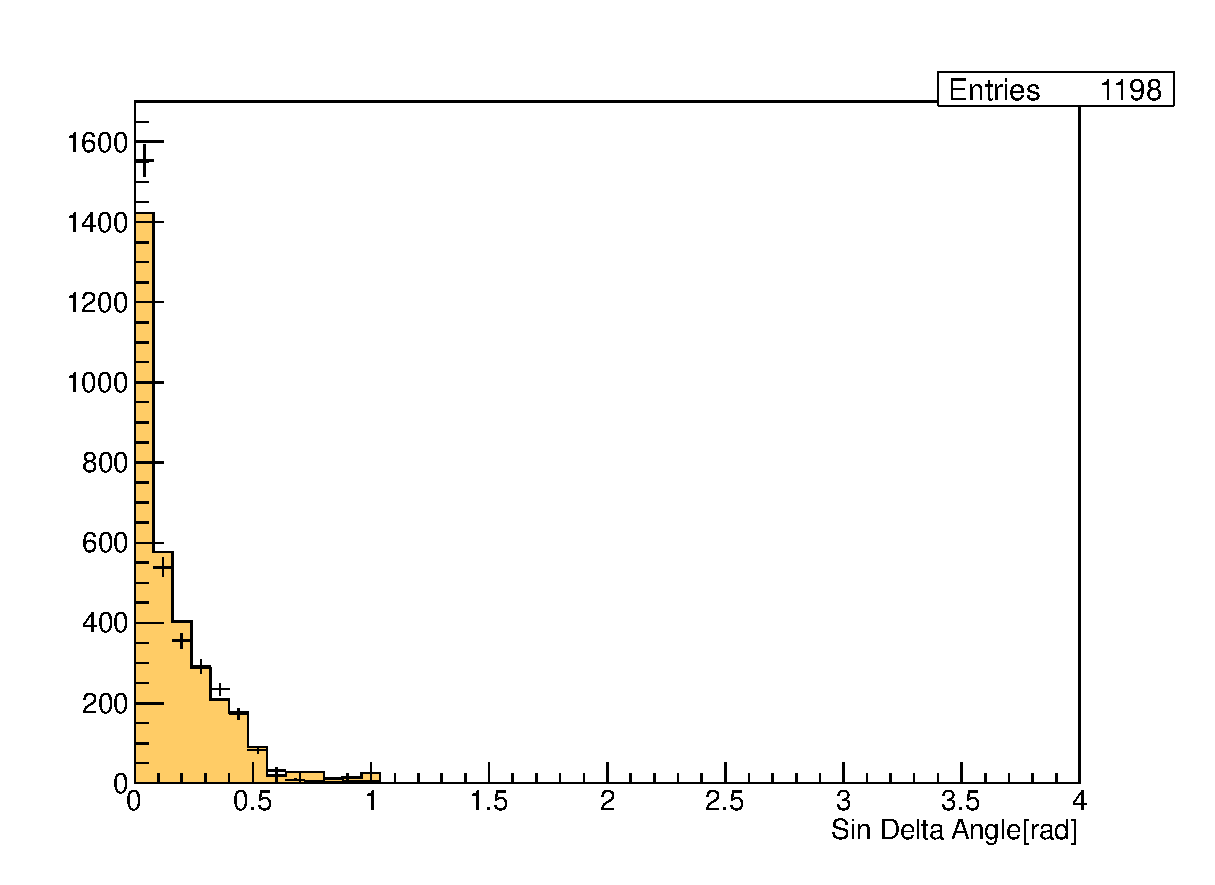
\includegraphics[width=3.25in]{Figures/Systematics/MatchingEfficiency/dScosmics.eps}
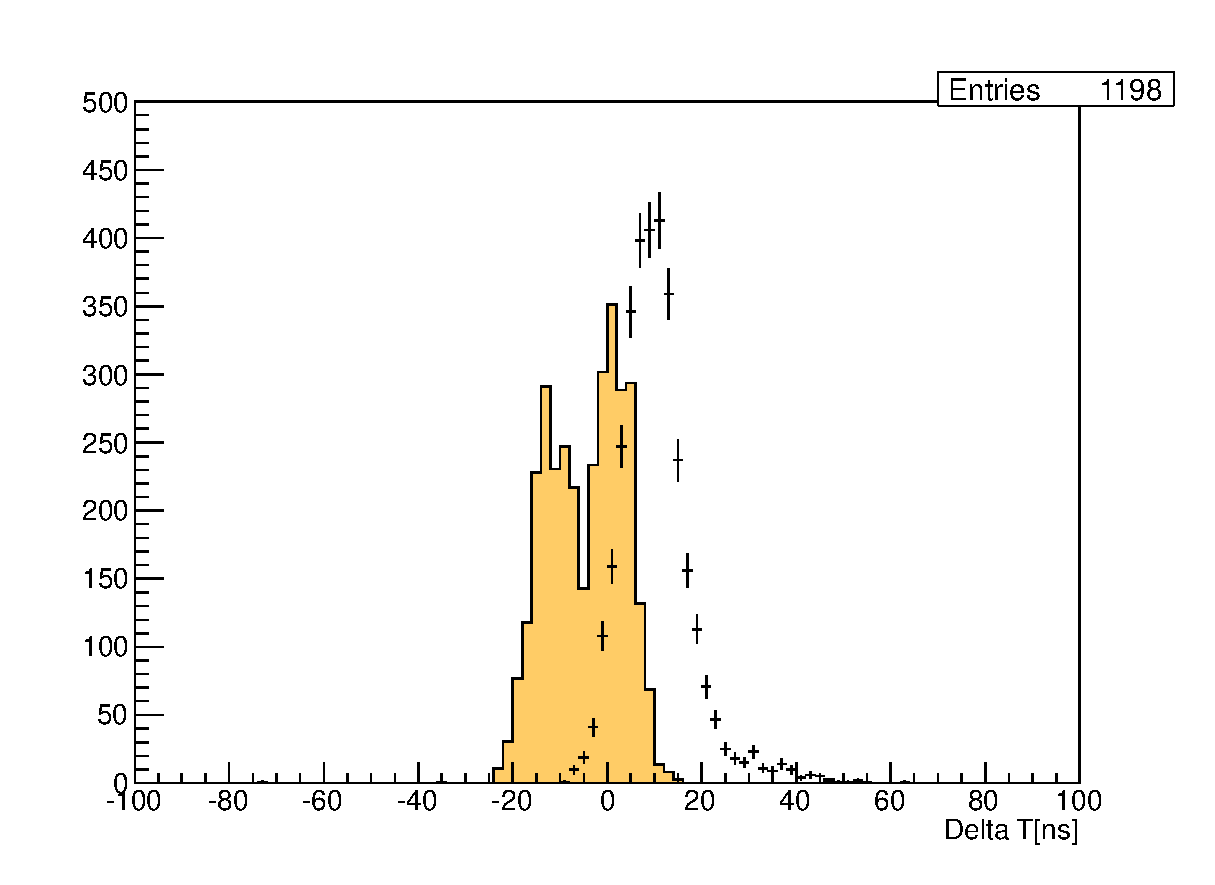
\includegraphics[width=3.25in]{Figures/Systematics/MatchingEfficiency/dTcosmics.eps}
\caption{Cosmics matching efficiency parameters \(\sin \theta\) and \(\Delta T\). The difference in \(\Delta T\) is not understood, but the cut is placed wide enough to be insensitive to the overall shift.}
\label{fig:eff_dSdT}
\end{figure}
\end{landscape}
}

\begin{figure}[h]
\centering
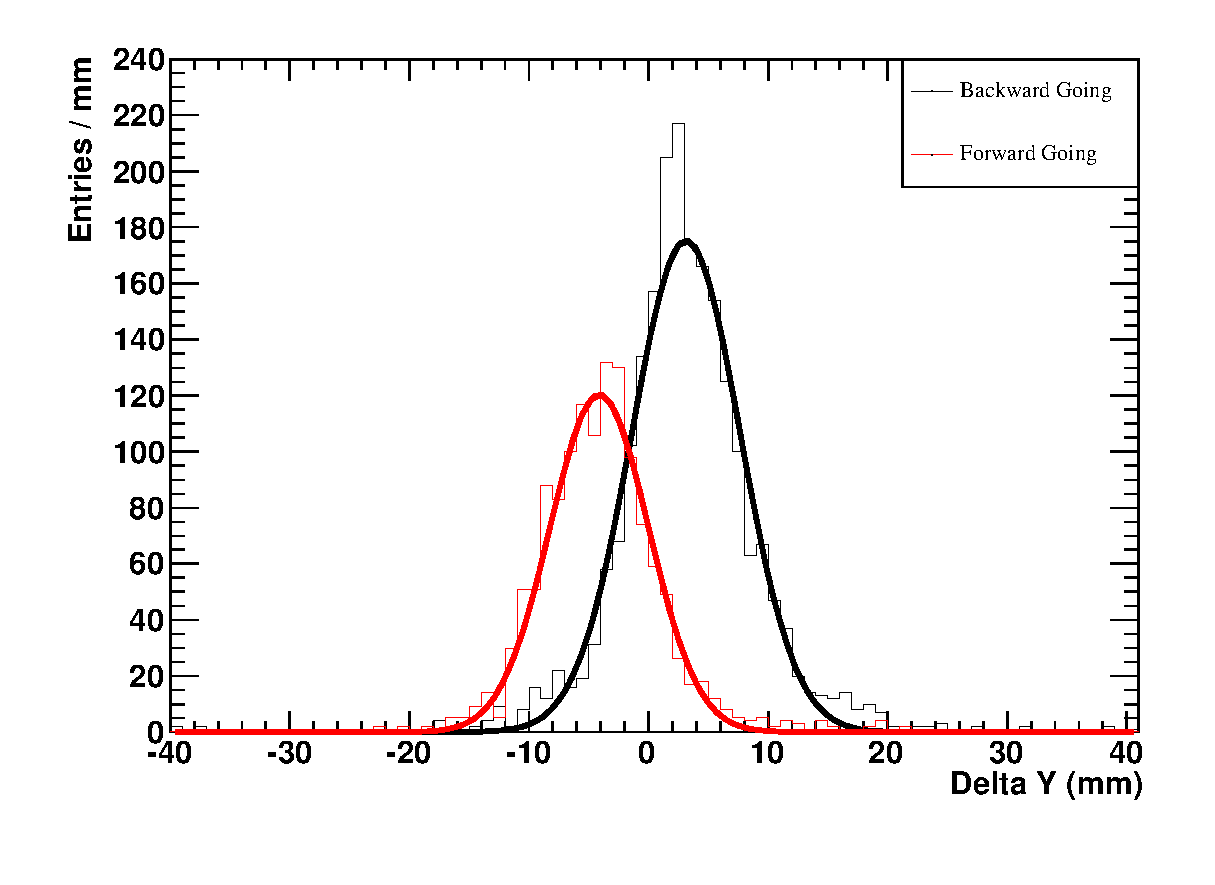
\includegraphics[width=3in]{Figures/Systematics/MatchingEfficiency/datadY.eps}
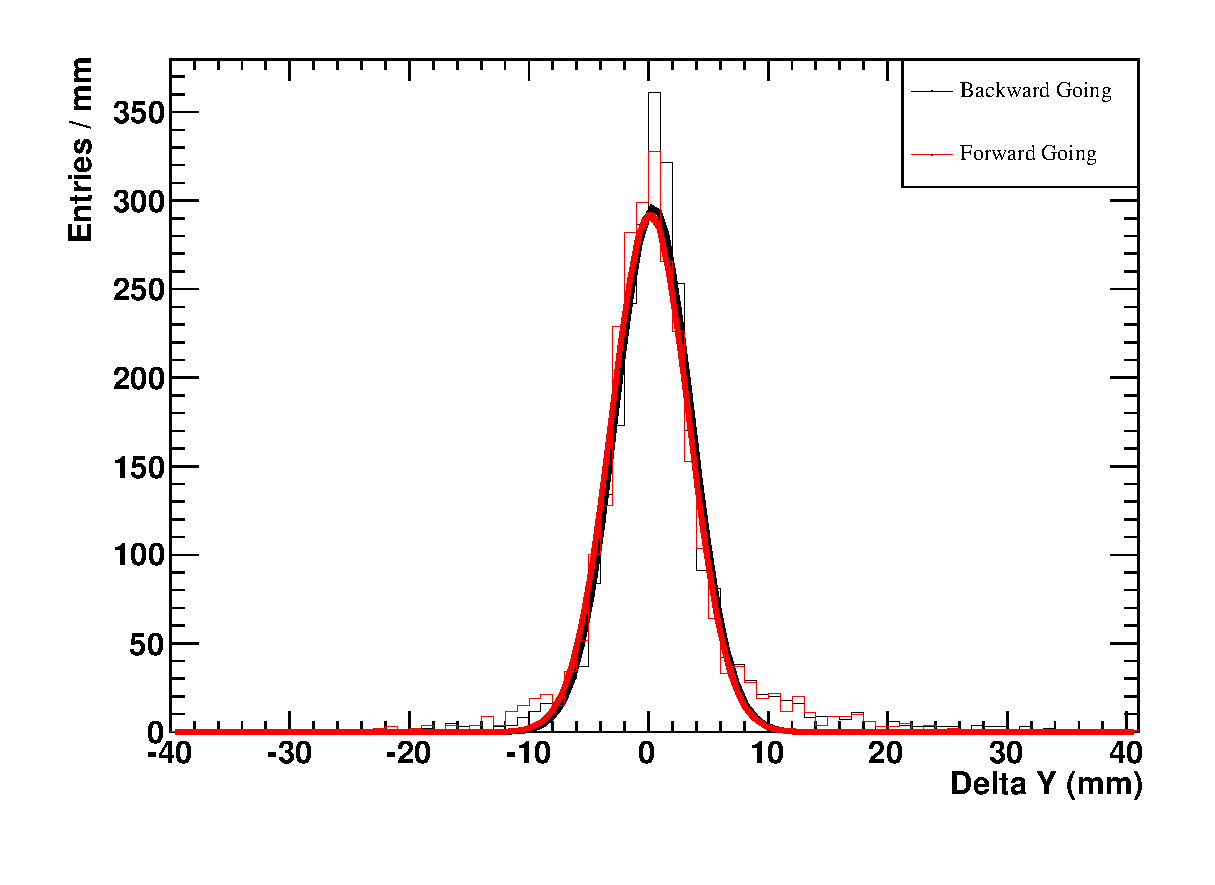
\includegraphics[width=3in]{Figures/Systematics/MatchingEfficiency/mcdY.eps}
\caption{
Matching Parameter $\Delta$ Y for FGD cosmics in data and MC split into forward and backward going tracks. Gaussian fits have been overlayed. The left plot shows the shift in the residual in data cosmics when comparing forward (red) and backward (black) tracks. The right plot shows that in MC we do not see such a shift between forward (red) and backward (black) tracks.
}
\label{fig:dY}
\end{figure}

\begin{table}[h]
\caption{Gaussian fit results and fit error of $\Delta Y$ for 10000 Production 4 FGD Cosmics in data and MC. The results are divided into backwards and forward going cosmics as determined by the Tracker reconstruction.}
\centering
\begin{tabular}{lccc}\toprule\midrule
Type and Dir. &  Mean & Sigma & $\chi^2$/NDOF \\ \midrule
Data Forward & $-4.1\pm 0.1$ & $4.1\pm 0.1$ & $100.0/48$  \\
\midrule
Data Backward & $3.1\pm 0.1$ & $4.5\pm 0.1$ & $155.2/58$ \\
\midrule
MC Forward & $0.1\pm 0.1$ & $3.2\pm 0.1$ & $255.1/51$ \\
\midrule
MC Backward & $0.5\pm 0.1$ & $3.2\pm 0.1$ & $263.2/59$ \\
\bottomrule
\end{tabular}
\label{tab:FitdY}
\end{table}

\begin{figure}
\centering
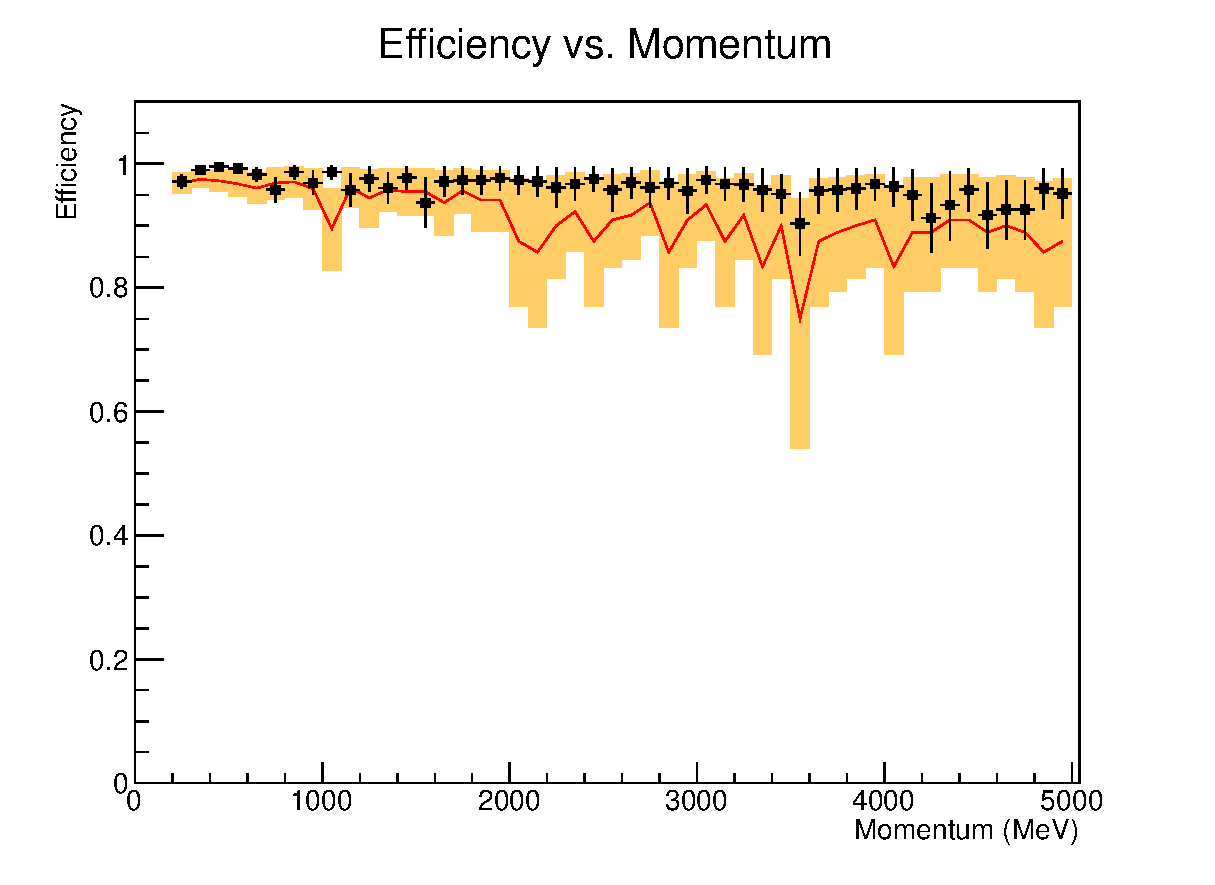
\includegraphics[width=3in]{Figures/Systematics/MatchingEfficiency/Eff_vs_Momentum.eps}
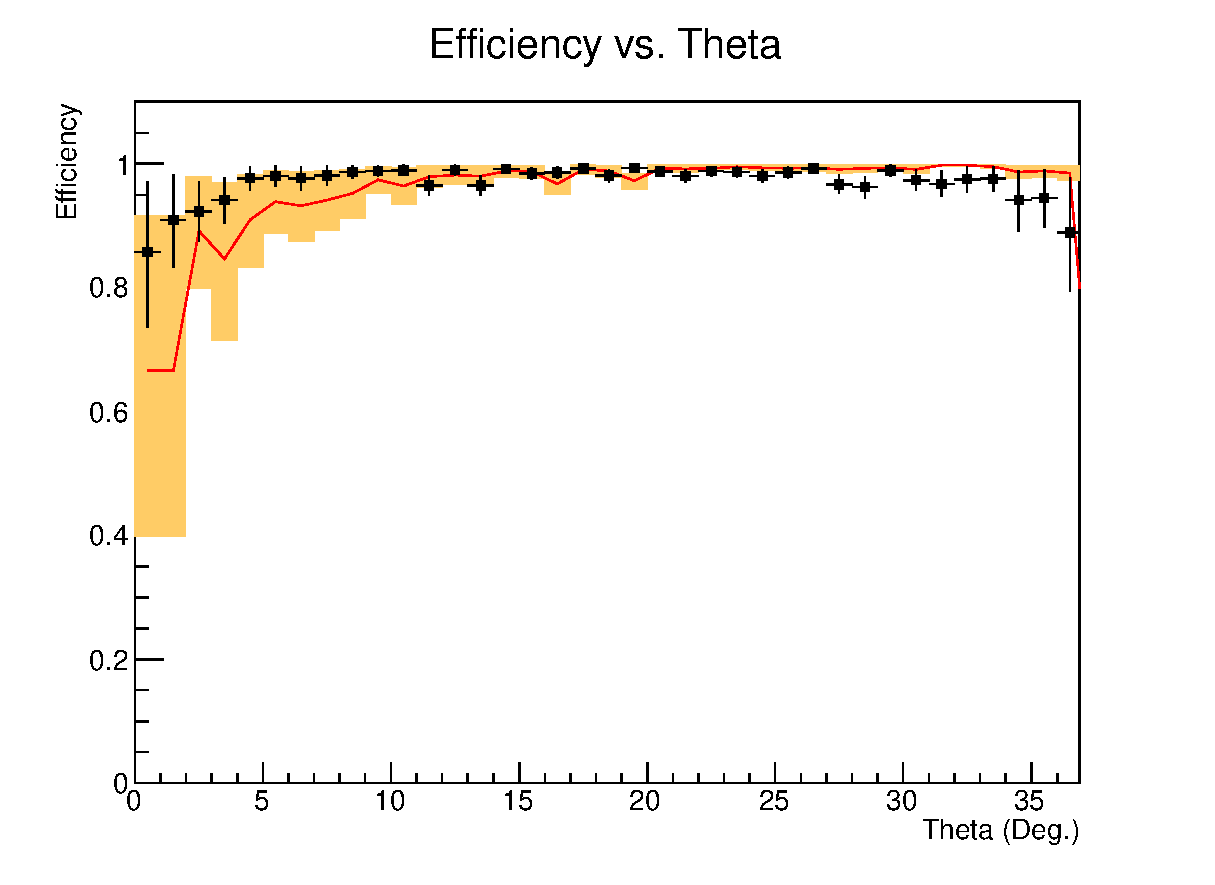
\includegraphics[width=3in]{Figures/Systematics/MatchingEfficiency/Eff_vs_Theta.eps}
\caption{Cosmics efficiencies as a function of Momentum and \(\theta\). Black dots are data and red line is the MC. The orange fill shows the error on the MC. We note that the data and MC efficiencies track each other as a function of both kinematic variables.}
\label{fig:eff_ND}
\end{figure}

Figure \ref{fig:eff_ND} then shows the final efficiency values for data and MC as a function of muon momentum and $\theta$. Note that in Figure \ref{fig:eff_ND}, the statistical errors are calculated using a probability distribution function derived with a Bayesian approach. The derivation of the PDF can be found in a paper by M. Paterno~\cite{bayes} and is implemented in ROOT under the TEfficiency class. The central values in Figure \ref{fig:eff_ND} are then the mean of the PDF (as opposed to the median). The statistical error for the integrated ratio is calculated more simply by approximating the efficiency as a binomial distribution. The efficiencies from the FGD cosmics sample are $99.08\%\pm 0.16\%$ for data and $99.22\%\pm 0.24\%$ for MC.

\subsubsection{Reconstruction Failures in Beam Events}

We also performed a search for unclassified reconstruction failures in beam events to account for any possible systematic effect missed by the FGD cosmics and sand muons study. Similar to the method in Section \ref{sec:CosmicsEfficiency}, beam events with one or two quality Tracker tracks pointing directly into the P0D were pre-selected. As the data has a large number of sand muons present, we also added a cut to veto these events. If more than two above-noise hits were found in the outer edges of the P0D coincident in time with the TPC1 track, we tag the event as a sand muon and exclude it. Of the remaining events, we filtered out those where the matching algorithm failed to find a suitable P0D track to match with the Tracker piece. Finally, the filtered events were examined by hand using event plotting software to identify any potential reconstruction pathologies previously missed.

When hand scanning filtered events, we founds several modes of failure, many of which were expected. For example, events which had short or partially reconstructed tracks in the downstream end of the P0D as well as events with no P0D constituent were missed by the matching algorithm for obvious reasons. Furthermore, some DIS-like events had large clusters of energy deposits in the P0D and were difficult to separate properly into tracks. These were also missed by the matching algorithm as expected. However, there were three classes of failure which, by eye, looked as if they should have been successfully matched. These we examined more closely.

First, we found events with multiple clean tracks passing into TPC1 which were missed by our algorithm. Further study showed this failure mode existed both in data and MC and was an expected effect. A P0D to TPC track matching amibiguity (due to design) causes a small portion of multi-track events to fail the matching algorithm. Second, we found another class of failed events where the P0D and Tracker tracks were well matched spatially, but separated widely in time ($\Delta T$ failure). Finally, the last failure mode were events where the P0D and Tracker tracks were mismatched in the XZ projection, a symptom of incorrect T0 extraction at the TPC1 reconstruction stage. An incorrect T0 calculation creates an offset in the TPC drift direction (XZ). Figure \ref{fig:mismatchexamples} shows examples of the $\Delta T$ and $T0$ failure modes.

\begin{figure}[h]
  \centering
  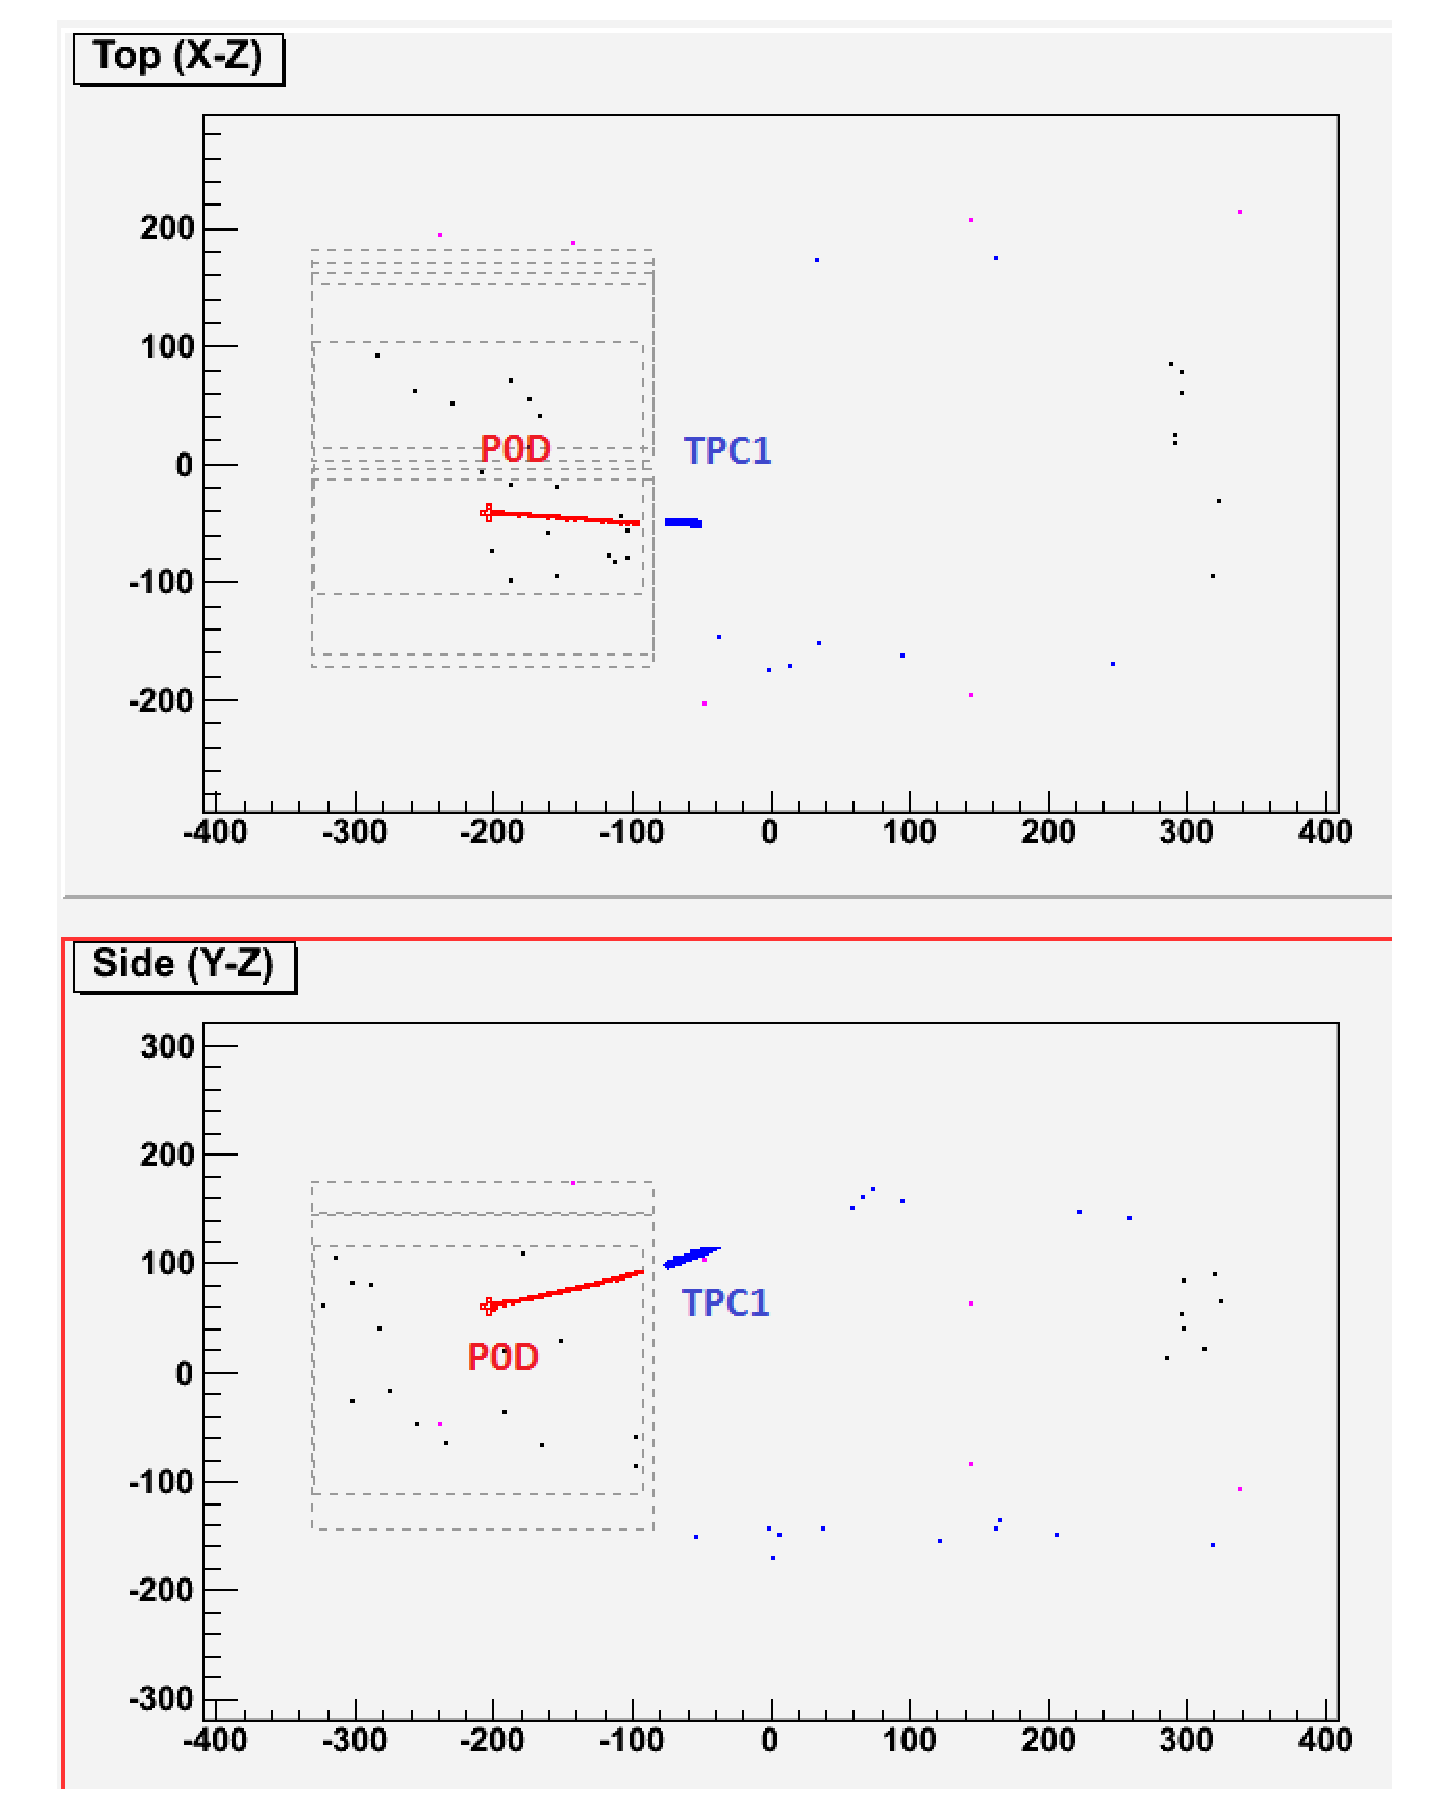
\includegraphics[width=3in]{Figures/delltaTmismatch.eps}
  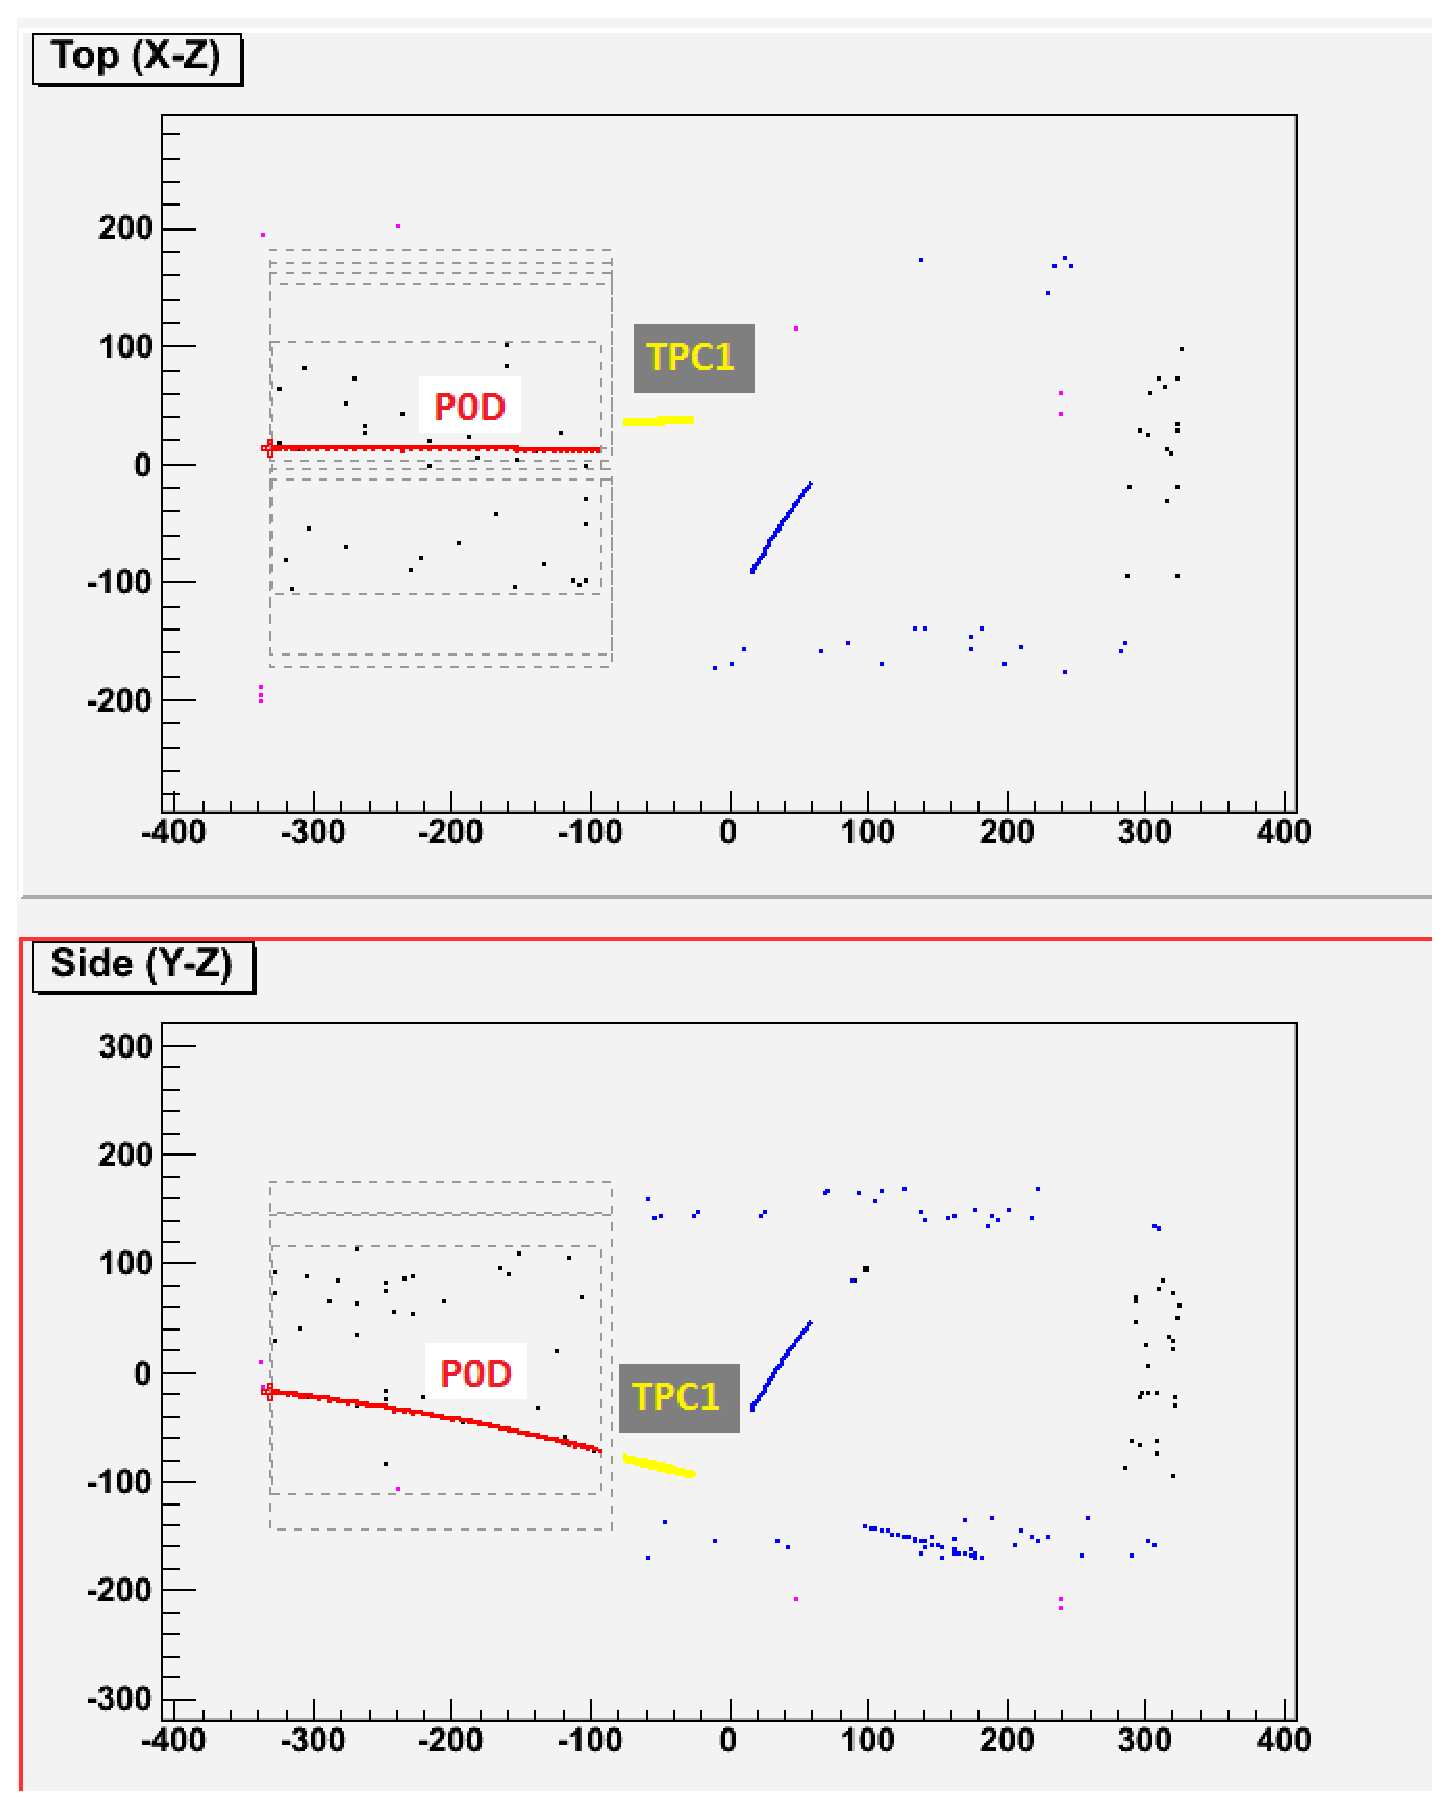
\includegraphics[width=3in]{Figures/t0mismatch.eps}
  \caption{An example of the $\Delta T$ (left) and $T0$ (right) failure modes. In the  $\Delta T$ failure, the P0D track (red) and the Tracker track (blue) match perfectly spatially, but are disjoint in time by $>100$ns. In the $T0$, the YZ projection has a good spatial match between the P0D track (red) and Tracker track (yellow), but the drift direction shows a symptomatic offset.} 
  \label{fig:mismatchexamples}
\end{figure}

We scanned by hand data events corresponding to $1.056\times 10^{19}$POT and MC events corresponding to $3.34\times 10^{18}$POT. The two timing related failure modes, $T0$ and $\Delta T$, were only observed in data and never in MC. Closer examination of the failed events showed that though some were muon-like tracks originating inside the P0D, many were actually sand muon events which made it through the veto. As the timing of the TPC1 track piece and the P0D track piece were generally different in these events, our sand muon veto did not associate the hits in the outer edges of the P0D with the TPC1 track, causing the sand muons to leak through our selection cuts. In Table \ref{tab:handscan} we summarize the number of events in data that failed via the $T0$ and $\Delta T$ modes and whether they originated from inside or outside the P0D.
\begin{table}[h]
\caption{
Total number of events from the $\Delta T$ and $T0$ failure modes for sand muons and in-P0D muon-like events.
}
\centering
\begin{tabular}{lcc}\toprule
& $\Delta T$ Failures & $T0$ Failures\\\midrule
Sand Muon & 11 & 20 \\
In-P0D Muon & 10 & 9 \\\bottomrule
\end{tabular}
\label{tab:handscan}
\end{table}

An examination of the $\Delta T$ failures show that none of the tracks have FGD constitutents. As the two control samples are predominantly tracks that pass through the FGD, the $\Delta T$ failure is most likely not accounted for in the efficiencies evaluated using Sand Muons and FGD Cosmics. We use the 10 $\Delta T$ In-P0D failures as uncertainty in the data event rate. 
Sand muon events which made it past our veto in this study would still be correctly rejected in the actual CC inclusive selection by the fiducial volume cut. However, the T0 effect is not necessarily replicated correctly in the cosmics and sand muon samples. When relatively steep tracks pass through TPC1 without also entering an FGD, the T0 is more likely to be miscalculated. Since FGD cosmics require the tracks to pass through the FGDs and sand muons are generally lengthy tracks passing through the entire ND280, T0 problems are less likely observed. So the hand scan study also adds a matching uncertainty due to the 9 muon-like tracks corresponding to the T0 failure mode. 

Including the statistical errors appropriately, we have $19\pm 4.36$(stat.) events more in the data from the T0 failure and the In-P0D $\Delta T$ failure modes combined. When normalized to the total data POT for each run type from the inclusive analysis, we get $422.28 \pm 96.88$  events per $23.47\times 10^{19}$POT for water-in running and $591.77 \pm 135.76$  events per $32.89\times 10^{19}$POT for water-out running.

\paragraph{Results of Matching Efficiency Systematic Studies}
\label{sec:Systematics_MatchingEfficiencyResults}

From the FGD cosmic sample, the MC / data efficiency ratio is $(99.22\%\pm 0.24\%) / (99.08\%\pm 0.16\%) = 100.14\%\pm 0.24\%$. This is the value we need to multiply the final data to MC ratio by to correct for efficiency. Similarly, using the results from the hand-scanning procedure, we calculate corresponding correction factors of $1.017 \pm 0.0039$ for water-in and $1.023 \pm 0.0053$ for water-out. These correction factors are multiplicative and uncorrelated with the cosmics efficiency correction. Propagating errors in quadrature yields total correction factors of $1.018 \pm 0.0049$ for water-in and $1.024 \pm 0.0060$ for water-out. The data to MC ratios are shifted by using this final correction factor. The corresponding errors are then $\pm 0.0049$ for water-in runs and $0.0060$ for water-out runs.


\subsection{Hit Reconstruction Efficiency}
\label{sec:Systematics_HitEfficiency}

We use a side-band sample of beam events to evaluate 
the layer by layer hit reconstruction efficiency in the P0D. The sample is generated by looking at events originating in the first layer of the P0D and is not a part of the actual selection. 
The hit reconstruction efficiency combines both the probability of finding an above threshold hit 
in a P0D bar with the probability of succesfully combining 
the hit into a track. 
As the P0D Reconstruction algorithm allows for gaps of hits in a track, 
we use particularly long reconstructed tracks to evaluate 
the rate of missed layers. 
Since each P0Dule has two layers (an X and a Y layer), 
we expect any track passing through a P0Dule to create 
two reconstructed nodes. 
So for each reconstructed track, we use the most upstream node 
and the most downstream node to calculate the number of total expected nodes. 
This value is compared to the number of actually reconstructed nodes. 
Then the efficiency per layer is given 
by: $($\# Expected Nodes - \# Reconstructed Nodes$)/($\# Expected Nodes$)$. 
To have similar levels of P0D bar coverage in both data and MC, 
we also require that any tracks used in this study begin and end at similar layer ranges. 
The hit reconstruction efficiency as a function of layer number 
is shown in Figure \ref{fig:hiteffsand}.

\begin{figure}
\centering
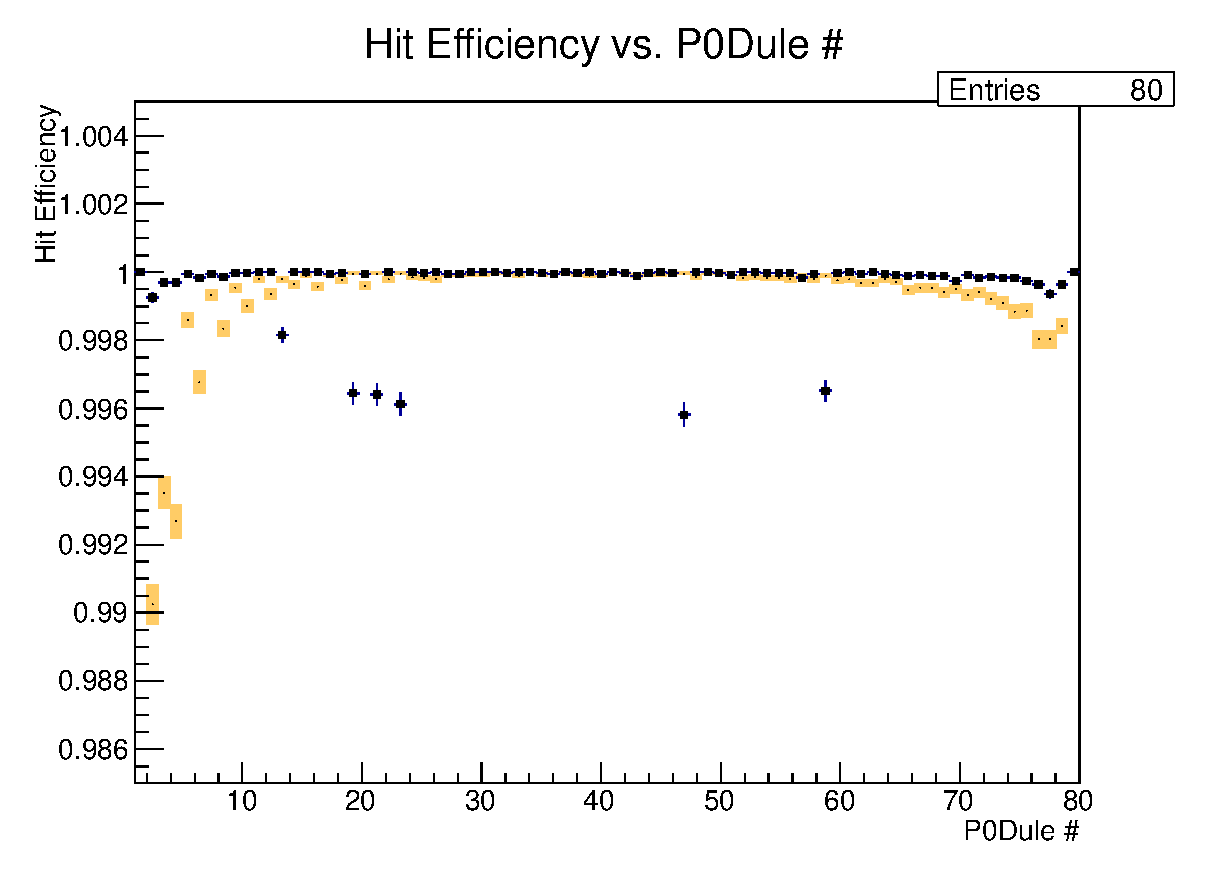
\includegraphics[width=3in]{Figures/Systematics/HitEfficiency/Hiteffsandw.eps}
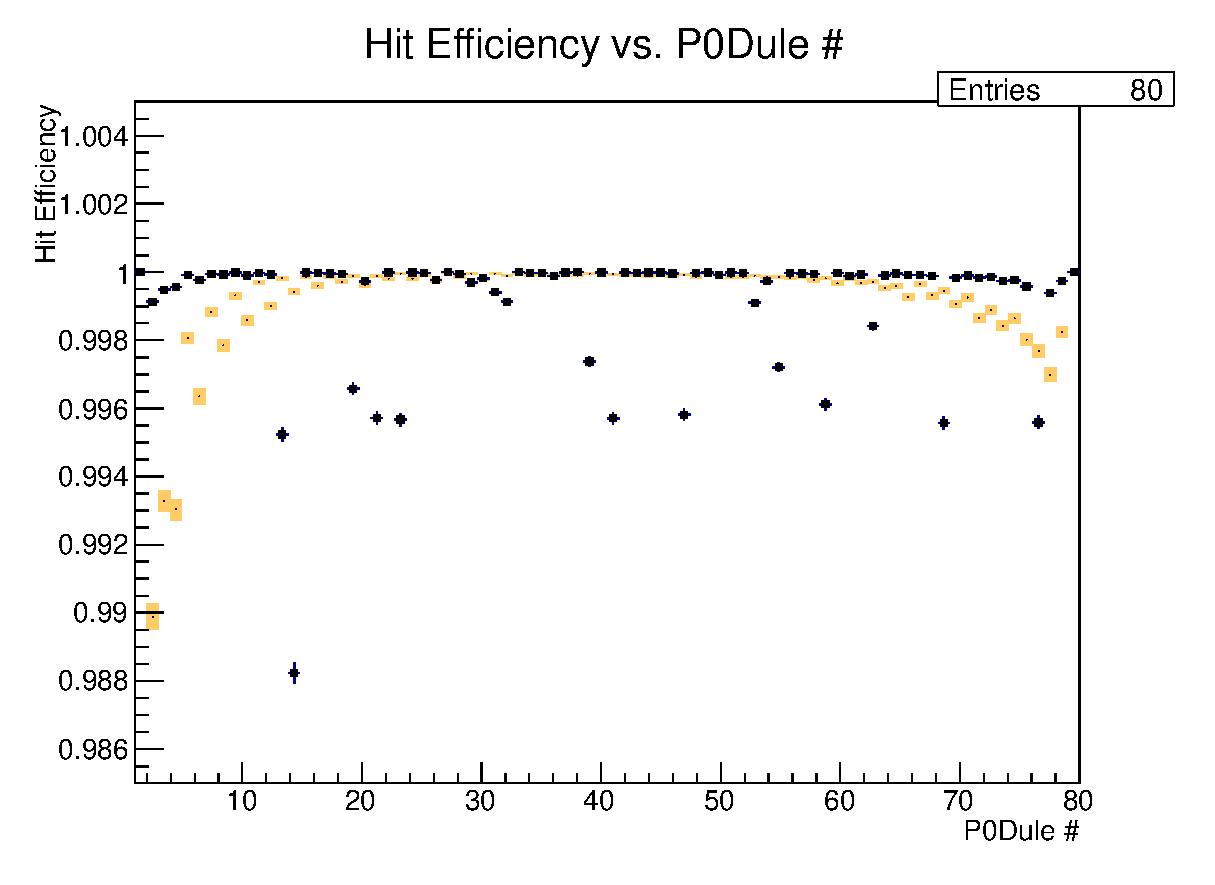
\includegraphics[width=3in]{Figures/Systematics/HitEfficiency/Hiteffsanda.eps}
\caption{The hit reconstruction efficiency as a function of layer number for water-in running (left) and water-out running (right). Data (black dots with error bars) and MC (orange error bars) show very high efficiencies for all layers. Layers corresponding to the water target have almost perfect efficiency. A few layers in the water target have ~0.5\% inefficiency. Note that the Y-axis is zero-suppressed.}
\label{fig:hiteffsand}
\end{figure}

\begin{table}
\caption{Data and MC hit reconstruction efficiencies by relevant layer numbers. Errors are excluded as the efficiencies are so high. }
\centering
\begin{tabular}{lcccc}\toprule\midrule
Layer \# &  Data (water-in). & MC (water-in) & Data (water-out) & MC (water-out)  \\ \midrule
15 & 1 & 0.999894 & 0.999984 & 0.999857 \\ \midrule
65 & 0.999916 & 0.999718 & 0.99996 & 0.999587 \\ \midrule
77 & 0.999638 & 0.998028 & 0.995591 & 0.997677 \\ \midrule
78 & 0.999359 & 0.998028 & 0.999394 & 0.996979 \\ \midrule
79 & 0.999638 & 0.998416 & 0.99975 & 0.998247 \\ \midrule
%80 & 0.994044 & 0.999141  \\ \midrule
\bottomrule
\end{tabular}
\label{tab:hiteff}
\end{table}

As expected, the hit reconstruction efficiency is extremely high. The few layers in data with small 0.5\% inefficiencies are at the single bar level, which are also expected. Any systematic arising from hit reconstruction efficiency will feed in through our matching algorithm and the fiducial volume cut. In the matching algorithm, we require that the P0D track have a node in the last two p0dules, so if both p0dules somehow failed to reconstruct a node, then we would have a small inefficiency. The last two p0dules correspond to layer numbers 77-80. Also, when making the fiducial volume cut, we may misreconstruct out-of-FV tracks as in-FV due to missed nodes at the upstream end of the water target. Similarly, we may lose in-FV tracks in the downstream end of the water target. Even in the least efficient of our p0dules, failing to reconstruct two or more adjacent nodes from a track is negligible (less than 0.0025\%), so we can estimate the effect of hit reconstruction efficiency on the fiducial cut using only the likelihood of missing a single node. The upstream end of the fiducial volume corresponds to layer 15 and the downstream end corresponds to layer 65. The hit reconstruction efficiencies for layers 15, 65, and 77-80 are given in Table \ref{tab:hiteff}.

From this table, we can then extract the final systematic values due to hit reconstruction efficiency. The probability of having \emph{no} nodes in the last two layers is essentially zero and therefore not included as a systematic. The probability of having gained an out-of-FV track from the upstream end of the FV cut is given by number of muon candidate tracks originating in layer 16 multiplied by the inefficiency of layer 15. Similarly, the probability of having missed an in-FV track at the downstream end of the FV cut is given by the \# of muon candidate tracks orginating in layer 66 multiplied by the inefficiency of layer 65. The largest inefficiency is that from layer 65 in MC water-out running, and it is 0.04$\%$. As the change in the data/MC ratio due to gains and losses of events from hit inefficiency cannot exceed this fraction, and is realistically smaller, we can neglect any systematic effect from hit efficiency differences between data and MC.

\subsection{Neutral Back Scattering}

There are a certain class of events where one or more layers in the middle of a track have no energy deposited. They may appear to be the result of layer inefficiencies studied in the previous section, but further investigation shows that is not the case. Some neutrino interactions end up creating a backwards going neutral particle as well as a forward going charged particle. The backwards traveling neutral particle converts in several layers upstream of the true interaction vertex. The hits from the resulting charged particle are grouped together with the forward going particle to create a long track with a significant gap in the middle. As this topology appears to be a single track, the vertex is actually incorrectly reconstructed at the most upstream layer. This effect might migrate the vertex far enough upstream to cause the event to fail the fiducial volume cut. In that case, not only would we expect a smaller selection inefficiency, we might also get a systematic shift in the data/MC ratio depending on how well neutral interactions are modeled in the MC. 

We examined several aspects of neutral back scattered events. To quantify the magnitude of this effect in data and MC, we calculated the fraction of tracks that had more than 1 missing layer between its most upstream layer and most downstream layer. The results are shown in Tables \ref{tab:NodeMissFractionsWaterIn} and \ref{tab:NodeMissFractionsWaterOut}. We also studied the location of the missing layers with respect to the beginning of the track. The vertex layer number is subtracted from the missed layer number and the resulting value is histogrammed and normalized to the total number of tracks examined. The results are shown in Figure \ref{fig:MisssedNodePerTracks} where it is clear that the second node is the most frequently missed node in these types of events. Given that a two-node pair corresponds to one P0Dule, it is not surprising that a converted neutral particle does not often have the energy to leave multi-P0Dule tracks. We also calculated the POT normalized number of tracks with missing layers and listed the results in Tables \ref{tab:TracksWithMiss0to20perPTWaterIn} and~\ref{tab:TracksWithMiss0to20perPTWaterOut}.

\begin{table}[h]
\caption{The fractions of tracks with more than 1 missed node 
for both data and MC water-in samples in the different run periods.}
\centering
\begin{tabular}{lcc}\toprule
      & &  Fraction of tracks \\
\cline{2-3}
Run 1 & Data & $1.63\%$  \\ 
      & MC & $1.90\%$  \\ 
\cline{2-3}
Run 2 & Data & $1.40\%$  \\ 
      & MC & $1.76\%$ \\ 
\cline{2-3}
Run 4 & Data & $1.39\%$  \\ 
      & MC & $1.80\%$ \\ 
\bottomrule
\end{tabular}
\label{tab:NodeMissFractionsWaterIn}
\end{table}

\begin{table}[h]
\caption{The fractions of tracks with more than 1 missed node 
for both data and MC water-out samples in the different run periods.}
\centering
\begin{tabular}{lcc}\toprule
      & &  Fraction of tracks \\
\cline{2-3}
Run 2 & Data & $1.55\%$  \\ 
      & MC & $1.83\%$  \\ 
\cline{2-3}
Run 3 & Data & $1.46\%$  \\ 
      & MC & $1.80\%$ \\ 
\cline{2-3}
Run 4 & Data & $1.65\%$  \\ 
      & MC & $1.80\%$ \\ 
\bottomrule
\end{tabular}
\label{tab:NodeMissFractionsWaterOut}
\end{table}

\begin{figure}
\centering
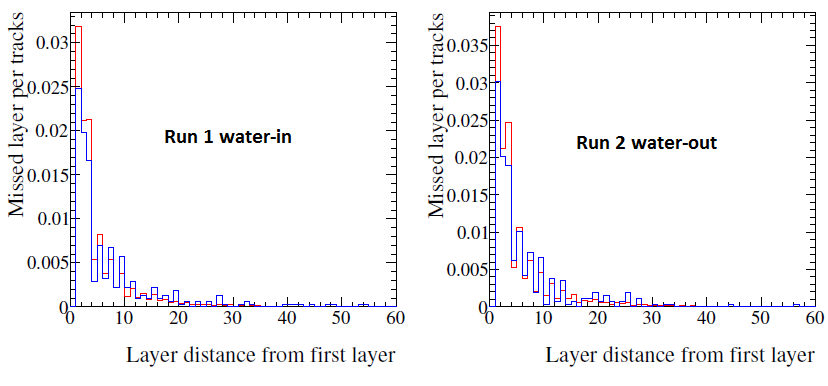
\includegraphics[width=5in]{Figures/layeff1.png}
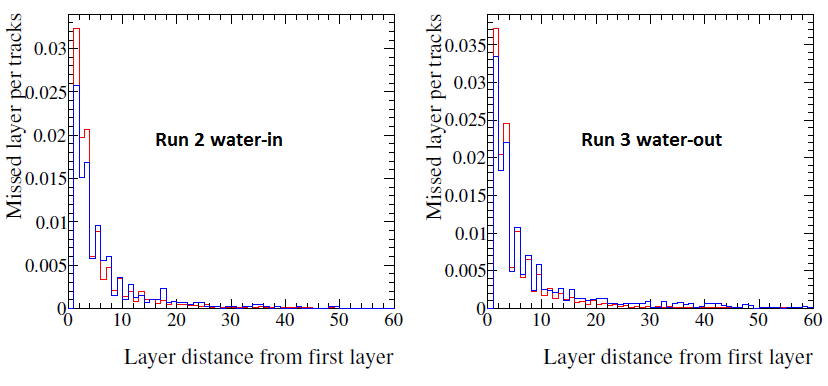
\includegraphics[width=5in]{Figures/layeff2.png}
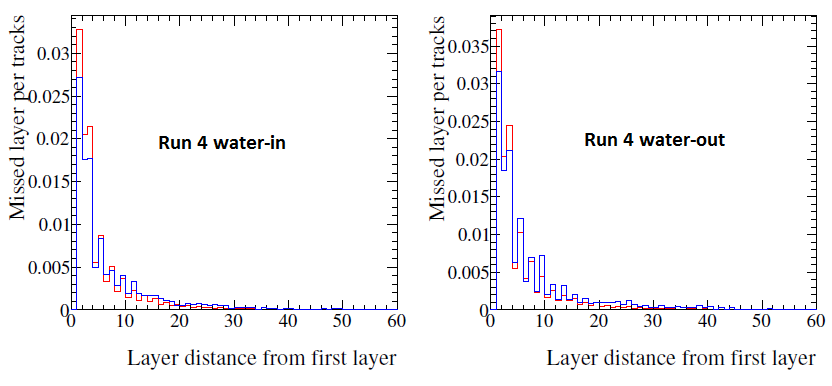
\includegraphics[width=5in]{Figures/layeff3.png}
\caption{The number of layers separating the first layer of missed nodes and the beginning of the track. The histograms are normalized to the total number of available tracks.
In all plots the blue and red histograms are generated from the data and MC samples
respectively.
}
\label{fig:MisssedNodePerTracks}
\end{figure}


\begin{table}[h]
\caption{The rate of tracks
with missed layers (layers 0 to 20 from counting from the start of the track)
for the data and MC water-in samples 
as calculated for run 1, run 2, run 4 and run 1$+$2$+$4 combined periods.
}
\centering
\begin{tabular}{lcc}\toprule
      & &  Tracks per POT [$\times 10^{-18}$] \\
\cline{2-3}
Run 1 & Data & $6.53$  \\ 
      & MC & $7.92$ \\ 
\cline{2-3}
Run 2 & Data & $7.13$  \\ 
      & MC & $8.08$ \\ 
\cline{2-3}
Run 4 & Data & $7.52$  \\ 
      & MC & $8.12$ \\ 
\cline{2-3}
Run 1+2+4 & Data & $7.32$  \\ 
      & MC & $8.09$ \\ 
\bottomrule
\end{tabular}

\label{tab:TracksWithMiss0to20perPTWaterIn}
\end{table}

\begin{table}[h]
\caption{The rate of tracks
with missed layers (layers 0 to 20 from counting from the start of the track)
for the data and MC water-out samples 
as calculated for run 2, run 3, run 4 and run 2$+$3$+$4 combined periods.
}
\centering
\begin{tabular}{lcc}\toprule
      & &  Tracks per POT [$\times 10^{-18}$] \\
\cline{2-3}
Run 2 & Data & $5.38$  \\ 
      & MC & $6.34$ \\ 
\cline{2-3}
Run 3 & Data & $6.14$  \\ 
      & MC & $6.34$ \\ 
\cline{2-3}
Run 4 & Data & $5.80$  \\ 
      & MC & $6.34$ \\ 
\cline{2-3}
Run 2+3+4 & Data & $5.90$  \\ 
      & MC & $6.34$ \\ 
\bottomrule
\end{tabular}
\label{tab:TracksWithMiss0to20perPTWaterOut}
\end{table}

Fortunately, despite the uncertain status of modeling neutral backscattering interactions, the data/MC ratios are unaffected. The fraction of tracks that suffer from missing layers is very low. Also, the absolute rate per POT of the occurence of this track topology is similar between data and MC. Finally, the distribution of missing nodes also tracks between data and MC quite well. All of this points to MC adequately simulating the effects of neutral particles backscattering. We assign no systematic error or correction due to vertex migration from backwards traveling neutral particles.

\subsection{Fiducial Volume Systematic}
\label{sec:fidvolsys}

There is a small possibility that the distribution of vertices is not properly simulated in the MC and that we somehow placed our fiducial boundaries where the vertex density is varying wildly. This would cause a systematic shift in the data to MC ratio that does not correspond to incorrect physics but rather incorrect detector simulation. It is however very unlikely that the vertex density varies very wildly right at the fiducial boundaries so any systematic effects are expected to be very small. To quantify this effect, we first evaluate the X and Y vertex reconstruction resolution with MC truth. The Z resolution is assumed to be 1 P0Dule layer. Any smearing of the Z direction resolution would be from hit inefficiencies or backwards going neutral tracks, situations that have been treated independently. To calculate the X and Y vertex position resolution, we simply take the residual of the reconstructed position and the true position of muon candidate tracks. Figure \ref{fig:fiducialResolution} shows the residuals fitted with a Breit-Wigner function. The X and Y vertex position residuals have a full width half maximum of 5.7~mm and 7.2~mm respectively.

\begin{figure}[ht]
\centering
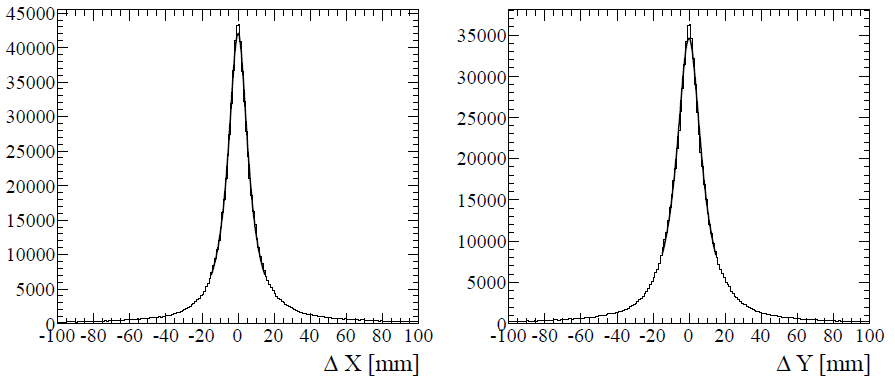
\includegraphics[width=5.5in]{Figures/Systematics/FVresolution.png}
\caption{Vertex position residuals of Reconstructed - MC truth for the X direction (left) and Y direction (right). This uses an arbitrarily large MC sample from run 1 with no applied normalization.} 
\label{fig:fiducialResolution}
\end{figure}

We take a conservative approach to evaluating the fiducial volume systematic. Given the FWHM of the X and Y position residuals, we vary the fiducial volume in those two axes by $\pm10$~mm. The Z axis fiducial boundaries are varied by one P0Dule layer. The CC inclusive selection is repeated twice for data and MC, once for the outward excursion of fiducial boundaries and once for the inward excursion. The outward excursion fiducial volume is define as the nominal volume plus 10~mm in X and Y and 1 layer in Z. Similarly, the inward excursion fiducial volume is the nominal volume minus 10~mm in X and Y and 1 layer in Z. The data to MC ratios are recalculated for each excursion and the difference from the nominal ratio is listed in Table \ref{tab:FVSystematic}. These values are a very conservative estimate of the systematic uncertainty associated with our fiducial volume boundaries.

\begin{table}[h]
\caption{The change in the nominal data to MC ratio when increasing and decreasing the selection fiducial volume by the assigned resolution values of each axis. Water-in and water-out samples were evaluated separately.}
\centering
\begin{tabular}{cccc}\toprule
 & & Water-in & Water-out \\ \midrule
Outside & & $+$0.00301 & $+0.00262$\\
Inside & & $-$0.00727 & $+0.00024$\\
\bottomrule
\end{tabular} 

\label{tab:FVSystematic}
\end{table}

There are a few other possible effects we must consider. One is the effect of hit reconstruction efficiency when making a FV cut. This has been shown to be negligible in Section \ref{sec:Systematics_HitEfficiency}. Another is the possibility that the vertex resolution in data is different from that in MC. However, we note that small differences in the width of the vertex resolution will not translate to a systematic uncertainty. The number of total true out-of-FV events that get `smeared' into the FV will cancel out with the number of true in-FV event that get `smeared' out of the FV. This statement requires two things to be true. First that the vertex resolution (i.e. the residual distribution) is symmetric, which we show is the case. Second, the underlying distribution of the true vertex distribution is flat near the fiducial volume boundaries. As the boundaries are set away from the physical edges of the water target, we find that the true vertex distributions are indeed flat. Finally, we note that the behavior of the vertex distributions in the selected sample are clearly not flat. This is due to selection inefficiencies and we correct for this in our cross section extraction. Whether the selection efficiency estimated by the MC can be trusted is investigated in this fiducial volume systematic section. Any differences between data and MC end up assigned as a systematic error.

Examining the matching parameter distribution (Figure \ref{fig:eff_dR}) from Section \ref{sec:CosmicsEfficiency}, we can draw some conclusions on the vertex resolution in data. The backwards projected Tracker track provides a best guess for where the true position of the P0D node should be, so the $\Delta Y$ and $\Delta X$ residuals mimic the vertex resolution. We see that the data and MC residuals have similar widths (see Table \ref{tab:FitdY} for an example) and more importantly, are symmetric. This indicates that vertex resolution has negligible effect on the Fiducial Volume systematic.

\subsection{Sand Muon Interference and Contamination}
\label{sec:sandintsys}

Muons that are generated by neutrinos interacting in the sand and concrete outside the ND280 are called ``Sand Muons''. These muons are often very energetic and can travel into and through the P0D. The sand muon veto step of the selection procedure is designed specifically to minimize the effect of this background source. While the veto does an excellent job in reducing the background, there are some subtleties when the same veto is also applied to the MC.

The simulation of data in the ND280 volume only uses the geometry of the detector out to the magnet yoke. This does not include any target mass in the form of the external concrete and sand where sand muons originate. To remedy the lack of simulated information from outside the detector itself, there is another MC sample with neutrino interactions solely in the sand. This however leaves out the unique case of coincidental sand muons and P0D water target interactions unsimulated. It is possible that a sand muon actually passed straight through the P0D while a signal neutrino interaction was occurring in water. This sand muon track may have then been mis-reconstructed as two broken track segments. This broken track then triggers our sand muon veto as one segment is considered as stopping inside the P0D even though the particle actually exited. This false veto causes a loss of efficiency in our selection and can also have a systematic effect on the data/MC ratio. We attempt to quantify the shift in the data/MC ratio, the error on the ratio and the level of contamination due to the sand muon background and its interaction with our veto strategy.

\subsubsection{Sand Muon Contamination}

Reconstructed sand muons occasionally cause false vetos of perfectly good CC inclusive events in the P0D, but there is another class of sand muon events that affect our analysis. A handful of times, an external sand muon has an erroneously reconstructed vertex within the water target fiducial volume and also enters the TPC. To the selection, these events are identical to a muon track from a CC inclusive interaction. This is a known background, but we also expect it to be extremely small. The likelihood of an external muon track being virtually undetected until the fiducial volume is miniscule. To quantify the magnitude of this background, we use the MC sand muon simulation discussed earlier. By applying the nominal CC inclusive selection to the sand muon simulation, we can estimate the expected sand muon contamination. For the water-in and water-out configurations of the detector, we find a sand muon contamination rate of 1.034 events per $10^{19}$ POT and 1.476 events per $10^{19}$ POT respectively. By normalizing these rates with the POT in a chosen sample, we have a MC based prediction of the sand muon contamination for all the runs. The percentages of sand muon contamination are shown in Table \ref{tab:sandcont}. As expected, the magnitude of this background mode is negligible. We do not assign any systematic error to this miniscule effect.

\begin{table}[h]
\caption{The percentage of selected events in each run that are expected to be external sand muons. These rates are based on a simulation of sand muons in water-in and water-out detector configurations.}
\label{tab:sandcont}
\centering
\begin{tabular}{cccc}
\toprule
Run & Water-in/out & Data & MC \\
\midrule
1 & Water-in & 0.00098 & 0.00088\\
2 & Water-in & 0.00094 & 0.00086\\
2 & Water-out & 0.00208 & 0.00214\\
3 & Water-out & 0.00198 & 0.00180\\
4 & Water-in & 0.00096 & 0.00087\\
4 & Water-out & 0.00180 & - \\
\bottomrule
\end{tabular}
\end{table}

\subsubsection{Sand Muon Interference}

To calculate the necessary correction to the data/MC ratio and the corresponding systematic error, we use a two step process. First, we use the sand muon simulation to estimate the probability of reconstructing an external sand muon track in the P0D in a single beam bunch. Then we use the beam MC and data and compare the fraction of events that pass the veto stage in each sample. This gives us a handle on any systematic differences we must account for in the ratio.

The probability having a sand muon track reconstructed in the P0D in a beam bunch can be written as

\begin{equation}
P_{bunch} = N_{sand} \times \frac{POT_{data}}{POT_{sand MC}} \times \frac{1}{N_{data spills}*N_{bunches}}
\end{equation}

In this equation, $N_{sand}$ is the number of beam spills that have at least one reconstructed P0D track. As this uses the sand muon only simulation, no tracks are expected from neutrino interactions inside the P0D volume. The POT terms represent the normalization of the probability to the exposure available in data. Finally, $N_{data spills}$ is the total number of cumulative beam spills in a given data sample and $N_{bunches}$ is the number of beam bunches in each data sample (6 or 8). This last term is the normalization of the probability to the total number of beam bunches available in a data sample. Using this equation, we can calculate the probability according to MC of reconstructing an external track in a beam bunch of a data sample. The results are shown in Table~\ref{tab:pbunch}.

\begin{table}[h]
\caption{The probability of reconstructing an external track in the P0D in a beam bunch as calculated from sand muon simulation.}
\label{tab:pbunch}
\centering
\begin{tabular}{ccc}\toprule
Run & Water-in/Water-out & $P_{bunch}$ \\
\midrule
1 & Water-in & 0.0125 \\
2 & Water-in & 0.0198 \\
2 & Water-out & 0.0232 \\
3 & Water-out & 0.0251 \\
4 & Water-out & 0.0279 \\
4 & Water-out & 0.0320 \\
\bottomrule
\end{tabular}
\end{table}

Next, we evaluate the fraction of events that survive the sand muon veto procedure in beam data ($R_{Data veto}$) and MC($R_{MC veto}$). Any differences in the survival rate ($R_{MC veto} - R_{Data veto}$) is nominally due to a difference in how often misreconstructed sand muons coincide with neutrino events in the water target. Table \ref{tab:rveto} shows the survival rates by run and type as calculated by dividing the number of events remaining after the veto by the number of events before. As expected, the majority of events survive even though the rate is not the same for data and MC. Since we expect the difference is due to the sand muon interference, the difference in survival probability in data and MC is used to calculate the systematic correction required on the central value of the absolute water cross section. This propagation is discussed later.

\begin{table}[h]
\caption{The fraction of events that survive the sand muon veto stage in data ($R_{Data veto}$) and MC ($R_{MC veto}$). The last column lists the difference between the theoretical probability of reconstructing an external track in the P0D ($P_{bunch}$ and the measured shift in survival rate in data and MC ($R_{MC veto} - R_{Data veto}$). This last value is used to calculate the systematic error on the sand muon interference correction.}
\label{tab:rveto}
\centering
\begin{tabular}{ccccc}
\toprule
Run & Water-in/Water-out & $R_{Data veto}$ & $R_{MC veto}$ & $P_{bunch}-(R_{MC veto}-R_{Data veto})$ \\
\midrule
1 & Water-in & 0.9822 & 0.9888 & 0.0059\\
2 & Water-in & 0.9829 & 0.9874 & 0.0152\\
2 & Water-out & 0.9632 & 0.9821 & 0.0043\\
3 & Water-out & 0.9748 & 0.9824 & 0.0175\\
4 & Water-in & 0.9767 & 0.9872 & 0.0173\\
4 & Water-out & 0.9653 & 0.9823 & 0.0150\\
\bottomrule
\end{tabular}
\end{table}

To evaluate the systematic error corresponding to sand muon interference, we compare the difference in survival rate with the probability of reconstructing an external track in the P0D in a single beam bunch ($P_{bunch}$). $P_{bunch}$ gives us an upper bound on the possible interference rate as not every single reconstructed external track is expected to cause a false veto in our selection. The survival rate difference ($R_{MC veto} - R_{Data veto}$) is used to calculate a correction to the cross section central value. We use the difference between $P_{bunch}$ and the survival rate shift to calculate the systematc error due to sand muon interference. This value is shown in the last column of Table \ref{tab:rveto} for the different runs. We increase/decrease the MC event rate by a factor of $P_{bunch}-(R_{MC veto}-R_{Data veto})$ and recalculate the data to MC ratio to get the upper/lower excursions. The difference between the nominal data to MC ratio and these two excursions yields the quoted systematic error from sand muon interference. The absolute $+1\sigma$ and $-1\sigma$ errors are shown in Table \ref{tab:sanderr}. The errors are propagated in a future section to the actual cross section measurement. 

\begin{table}[h]
\caption{The $\pm 1\sigma$ absolute errors for the water-in and water-out samples. The calculation of these values is described in the text.}
\label{tab:sanderr}
\centering
\begin{tabular}{ccc}
\toprule
Error Boundary & Water-in & Water-out \\
\midrule
$+1 \sigma$ & -0.0116 & -0.0144 \\
$-1 \sigma$ & +0.0119 & +0.0138 \\
\bottomrule
\end{tabular}
\end{table}

\subsection{Out of Fiducial Volume Systematic}

A fraction of selected CC inclusive events originate outside the fiducial volume and are misreconstructed inside. This Out of fiducial volume background (OOFV) must be evaluated in data and MC to see if there is any systematic difference in contamination rates. To do so, we first define four non-intersecting volumes near the P0D where candidate events might originate. 

\begin{enumerate}
\item WT Fiducial: Events in this region are signal as this is the target we are interested in.
\item CECAL$+$ no truth info: The CECAL is the volume directly downstream of the WT fiducial volume. Events from this region have backscattered into the water target volume to cause the reconstructed vertex to migrate upstream of the true position. This is the largest source of OOFV background. As we will be using MC for parts of this study, we also include all events without truth information in this event class. This decision is a conservative one as the CECAL volume has the largest BG contribution.
\item Inside P0D but outside CECAL: This volume covers all events that occured within the P0D but not within the CECAL. This volume is also outside the water target fiducial volume. They are primarily two types of events. The first kind occurred upstream of the water target but had some missed hits that cause the reconstructed vertex to migrate into the fiducial volume. The second kind are steep tracks originating around the edges of the water target that pass through enough dead material (water bags for example) to avoid proper vertex reconstruction.
\item Outside P0D: All other events are considered in this volume. Selecting such events is very unlikely and this background source is mostly events from the surrounding P0D Ecal and SMRD. 
\end{enumerate}

Using beam MC simulation, we calculate the fraction of selected CC inclusive candidates with a true vertex in these four volumes. The percentages are shown in Table \ref{tab:oofvfrac}. To calculate a systematic uncertainty on the data to MC ratio, we must ideally convolute this fraction with the data to MC CC inclusive event rate ratios from each region. However, volume 3 is an exception to the case. The reason OOFV events in this volume are being reconstructed in the fiducial volume is vertex smearing from hit inefficiencies and from the presence of dead material. We found that the X and Y vertex resolutions are symmetrica. We also found that the underlying MC vertex distribution is flat as a function of X and Y vertex position. This implies that the fraction of events lost from inside the fiducial volume due to this reason is roughly the same as the background entering the fiducial. So we do not include events from volume 3 in our OOFV systematic calculations.

\begin{table}[h]
\caption{The percentage of selected events in each run with true vertices in four predefined volumes. Volume 1 is signal, the rest are considered out of fiduial volume background. As these are calculated from MC, we do not have an independent run 4 water-out sample.}
\label{tab:oofvfrac}
\centering
\begin{tabular}{cccccc}
\toprule
Volume & Run 1 water-in & Run 2 water-in & Run 2 water-out & Run 3 water-out & Run 4 water-in \\
\midrule
1 & 96.70\% & 96.74\% & 95.70\% & 95.44\% & 96.75\%\\
2 & 2.05\% & 2.09\% & 2.69\% & 3.12\% & 1.96\%\\
3 & 1.14\% & 1.03\% & 1.38\% & 1.19\% & 1.16\%\\
4 & 0.11\% & 0.14\% & 0.23\% & 0.25\% & 0.13\%\\
\bottomrule
\end{tabular}
\end{table}

For the CECAL volume, we use a CC inclusive selection that is nearly identical to the nominal selection. The only difference is that the volume cut used is shifted into the CECAL. The X and Y boundaries are kept the same but the Z boundaries are shifted downstream to (-1266~mm,~-1016~mm). Events are selected from this slice of the CECAL in data and MC and the ratio of event rates is calculated. For the data to MC ratio in volume 4, we refer to a CC inclusive selection performed in the SMRD \cite{smrdtn} that reports a data to MC ratio of 1.085.

To calculate the systematic errors from volume 2 and volume 4, we first use the OOFV background fractions from Table \ref{tab:oofvfrac} to estimate the number of events in data that originated in each volume. The predicted number of data events from each volume is then multiplied by the data to MC ratio from that volume. This yields the corrected number of OOFV background events from each volume. Finally, the corrected OOFV background is subtracted from the original data total from the fiducial volume and the overall data to MC ratio is recalculated. The difference between the recalculated data to MC ratio and the nominal ratio, shown in Table \ref{tab:oofv}, is used as ths systematic error due to the OOFV background. The results from the different runs are combined by averaging after POT-weighting. The OOFV systematic error from volume 2 and volume 4 combined yields $\pm0.000274$ and $\pm0.000537$ for the water-in and water-out samples respectively.

\begin{table}[h]
\caption{The out of fiducial volume systematic difference between data and MC from events in Volume 2 and Volume 4 for different runs. The final two rows are the combined systematic shifts for the water-in and water-out (air) samples as calculated by POT-weighted averaging.}
\label{tab:oofv}
\centering
\begin{tabular}{cccc}
\toprule
Run & Water-in/out & Volume 2 & Volume 4 \\
\midrule
1 & Water-in & 0.000028 & 0.000207\\
2 & Water-in & 0.000775 & 0.000249\\
2 & Water-out & 0.000480 & 0.000492\\
3 & Water-out & -0.000873 & 0.000457\\
4 & Water-in & -0.000007 & 0.000236\\
4 & Water-out & -0.000242 & 0.000480 \\
1+2+4 & Water-in & 0.000141 & 0.000235 \\
2+3+4 & Water-out & -0.000242 & 0.000480 \\
\bottomrule
\end{tabular}
\end{table}

\subsection{Event Pile-up Systematic}

Our selection only allows a single neutrino interaction per beam bunch. If there were multiple CC interactions within the same integration window, we only select the one that produced the higher momentum muon. The probability of multiple interactions is very low considering the magnitude of the CC inclusive cross section, so we do not expect a large event pile-up effect. However, since the beam power (and therefore the neutrino flux per time) changes for various practical reasons, the MC can never perfectly simulate the event pile-up rate. If the pile-up rates are drastically different between data and MC, then the ratio will be systematically shifted. To evaluate the magnitude, we first assume that there is an equal probability for an interaction to occur in a given beam bunch. This is a reasonable assumption as the beam power does not change appreciably over each spill. Then we take the number of bunches that had a candidate CC event and divide by the total number of bunches where an event may have occurred. The latter value is nominally the number of beam bunches per spill (6 for run 1 and 8 for all others) multiplied by the total beam spills in each run. This yields the probability of reconstructing a CC candidate event in any given bunch. The square of this probability is the event pile-up rate, i.e. the chance of two events occurring in the same beam bunch. This rate was found to be on the order of $1\times 10^{-7}$l and so no systematic error was assigned due to the event pile-up effect.

\subsection{Track Timing Systematic}

In the event we placed our timing cut in a place where the data and the MC time distributions are very different in shape, we expect a systematic shift in the data to MC ratio. However, the timing of beam induced events peaks at well known time stamps with a very narrow width. Our timing cuts are also placed quite wide, using up a large fraction of what is allowed by the electronics. The expected effect from reconstructing stray tracks outside the time cuts is extremely low. To cross check this expectation, we vary the time cuts in a similar manner to the fiducial volume systematic evaluation. The time windows are widened and narrowed by 15~ns and 18~ns for run 1 and run 2 respectively. These variation values are the bunch-averaged peak widths of the time distribution of muon candidates. The timing variation found no change in run 1 and only a single event that failed the inside excursion of the timing cut in run 2. The process was not repeated for run 3 or run 4 as these values prove that there is negligible effect of shifting the timing cut. No systematic error is assigned to this source.

\subsection{Cosmic Background Systematic}

While our beam data includes the possibility of reconstructing cosmic events, our beam MC sample does not include any type of cosmic flux. This implies that the data event rates must be corrected for any cosmic event contamination. To measure the contamination, we use a sideband sample from our available beam data. There are a few empty electronics integration cycles before the 6 or 8 integration cycles when the beam arrives. We argue that any events reconstructed in these nominally empty integration cycles are entirely from the cosmic background. So we search these integration cycles for any events that pass our CC inclusive selection and then divide the total selected tracks by the amount of time these integration cycles were open. The cosmic tracks per unit time value is then multiplied by the total amount of time within our beam selection time cuts to calculate the predicted cosmic contamination rate in our beam data. The results from run 1 and run 2 are summarized in Table \ref{tab:cosmiccont}. We did not process any of the other runs as the expected cosmic contamination are so small that this background channel is negligible. So it follows that no systematic correction or error is assigned to the data event rate because of the cosmic background.

\begin{table}[h]
\caption{Expected cosmic contamination rates in run 1 and run 2. The contamination rates are not POT normalized.}
\label{tab:cosmiccont}
\centering
\begin{tabular}{ccc}
\toprule
 & Run 1 & Run 2\\
\midrule
Selected cosmic tracks & 2 & 0\\
Total cosmic search time & $2.429\times10^9$~ns & $2.811\times10^9$~ns \\
Total allowed beam time & $2.159\times10^9$~ns & $3.331\times10^9$~ns \\
Expected cosmic BG & 2 tracks & 0 tracks\\
\bottomrule
\end{tabular}
\end{table}

\subsection{TPC1 Tracking Efficiency}
\label{sec:Systematics_TPC1tracking}

When calculating the P0D tracking and matching efficiency in Section \ref{sec:matchingsyst}, we used a selection of tracks which were reconstructed in TPC1. In this section, we now evaluate the systematic uncertainty arising from the efficiency of reconstrucing a track in TPC1 using sub-detector reconstruction only. 

The technique uses a selection of events with reconstructed tracks in the P0D and TPC2 and looks for the fraction of time where there is also a reconstructed track in TPC1 \cite{trkefftn}. Any TPC1 track found is required to have at least 18 nodes, a quality cut used in most T2K tracking analyses. The required TPC2 track, called a reference track, is required to be 60 nodes long. The P0D reference track is required to be at least 72~cm long and have energy deposited in the most downstream layer. The 72~cm cut is selected to provide roughly the same solid angle distribution as the TPC2 reference tracks. The P0D reference track is helically extrapolated to the Z position of the TPC1 upstream face. If the X and Y positions of the projected point are within the X and Y limits of the TPC1 upstream face, then the algorithm passes to the next cut. The TPC2 reference track is extrapolated backwards to the downstream face of the P0D. If the extrapolated TPC2 track intersects the downstream face of the P0D within 200~mm of the exit point of the P0D reference track, then there is an expected track in TPC1. Exactly the same procedure is repeated for data and MC.

The efficiencies, binned by track momentum, are shown in Figure \ref{fig:tpc1eff}. We find the TPC1 tracking efficiency to be very high and the uncertainty very low so we linearly add the central \textit{in}-efficiency ratio value with the error to calculate the final systematic. 

\begin{figure}[h]
\centering
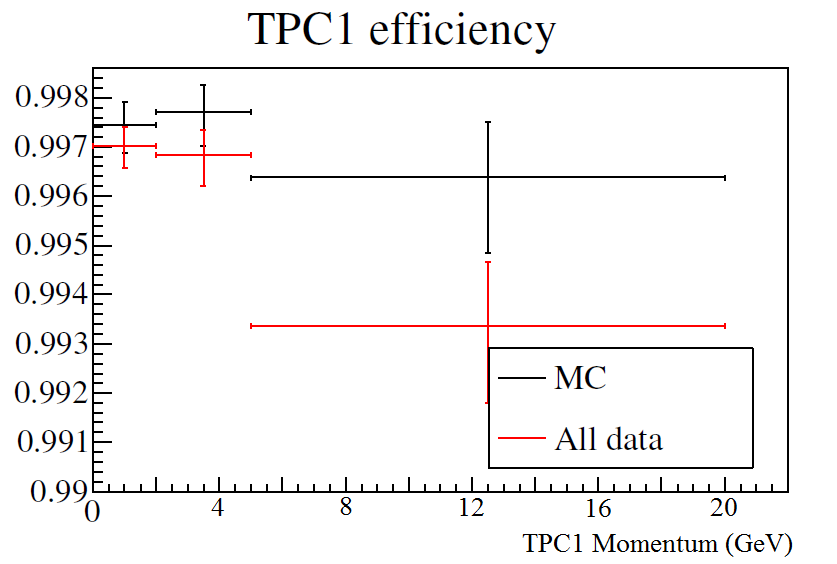
\includegraphics[width=4in]{Figures/tpc1matcheff.png}
\caption{TPC1 Track Finding Efficiency vs. muon momentum from 0~GeV to 20~GeV. Black (Red) shows MC (data). The plot is zero suppressed.}
\label{fig:tpc1eff}
\end{figure}

\begin{table}[h]
\caption{TPC1 Track finding efficiencies and ratios of efficiency for MC and data. Errors are also shown. All numbers are percentages.}
\label{tab:tpc1eff}
\centering
\begin{tabular}{cccccc}\toprule
& MC & Data & Ratio & \% Water-in & \% Water-Out \\ \midrule
0 - 2 GeV & $99.74 \pm 0.05 \%$ & $99.70 \pm 0.04 \%$ & $99.96 \pm 0.07 \%$ & 57.1 \% & 57.3 \% \\
2 - 5 GeV & $99.77 \pm 0.06 \%$ & $99.68 \pm 0.06 \%$ & $99.91 \pm 0.09 \%$ & 31.5 \% & 25.1 \% \\
5 - 20 GeV & $99.64 \pm 0.14 \%$ & $99.34 \pm 0.14 \%$ & $99.70 \pm 0.20 \%$ & 11.4 \% & 8.1 \%\\
\bottomrule
\end{tabular}
\end{table}

The TPC1 efficiency results are shown in Table \ref{tab:tpc1eff}. Linearly adding the inefficiency ratio and error, 
the TPC study obtains very small uncertainties of 0.1\%, 0.2\% and 0.5\% 
for momentum bins 0-2 GeV, 2-5 GeV and 5+ GeV respectively. 
These uncertainties are then weight-averaged with the percentage 
of selected events in each momentum bin for each run type. 
The systematic yielded by this study for a single momentum bin is $0.18 \%$ for water-in and $0.15 \%$ for water-out. 
As expected, the overall effect from tracking inefficiencies 
in the TPC is extremely small.

\subsection{Charge Mis-ID}
\label{sec:Systematics_ChargeMisID}

Occasionally, the TPCs fail to properly reconstruct the charge of a track. This reconstruction failure can cause our selection to either falsely identify muon tracks or fail to select a muon track that was mistakenly tagged as positive. To evaluate how often the charge of a track is misidentified, simultaneous charge measurements of a single track from TPC1 and TPC2 are compared \cite{chmisidtn}. The probability of TPC1 and TPC2 measuring the same charge ($P_{same}$), regardless of whether it is correct, is related to the probability of a single TPC incorrectly reconstructing the charge as follows:
\begin{eqnarray*}
P_{same} & = & P^2_{r} + P^2_{w} \\
P_{same} & = & (1-P_{w})^2 + P^2_w \\
P_w & = & \frac{1}{2}\left( 1- \sqrt{1-2(1-P_{same})} \right)
\end{eqnarray*}

Here $P_r$ is the probability of a single TPC reconstructing the correct charge and $P_w$ is the probability of a single TPC reconstructing the wrong charge. It has been assumed that the mis-ID probability $P_w$ is the same for both TPC1 and TPC2. As $P_{same}$ is rather trivial to measure in data and MC, we now have a simple way to calculate the charge mis-ID probability $P_w$. To cross check the charge mis-ID values calculated this way, the true charge information from the MC is used. Figure \ref{fig:chmisid} shows the charge mis-ID rate vs. track momentum. The probability method refers to the technique of calculating $P_w$ from $P_{same}$ and the charge method refers to the calculation of the mis-ID rate directly from the MC truth. Other than the expected correlation between mis-ID rate and track momentum (and therefore track curvature), we also note that the three methods are in agreement.

There is one final subtlety in calculating the correct charge mis-ID rate. The probability method requires the comparison of TPC1 and TPC2 charge measurements of the same track. Whether the track in TPC1 and TPC2 is the same is determined by a matching algorithm, which can of course fail sometimes. This failure to match together the correct pair of tracks means that there is no reason to expect both the TPCs to reconstruct the same charge and the equation for $P_w$ no longer applies. To correct for this subtlety, MC truth is used to calculate the fraction of times where a track charge is misreconstructed due to track mismatching. The charge mis-ID rate from track mismatching is then subtracted from the total charge mis-ID rate $P_w$ calculated by the probability method. The mis-ID rate due to track mismatching is also shown in Figure \ref{fig:chmisid}. The corrected charge mis-ID rates used to evaluate the systematic uncertainty in our analysis is listed in columns~2 and~3 in Table \ref{tab:N_corr_w} for water-in and Table \ref{tab:N_corr_a} for water-out.

\begin{figure}[h]
\centering
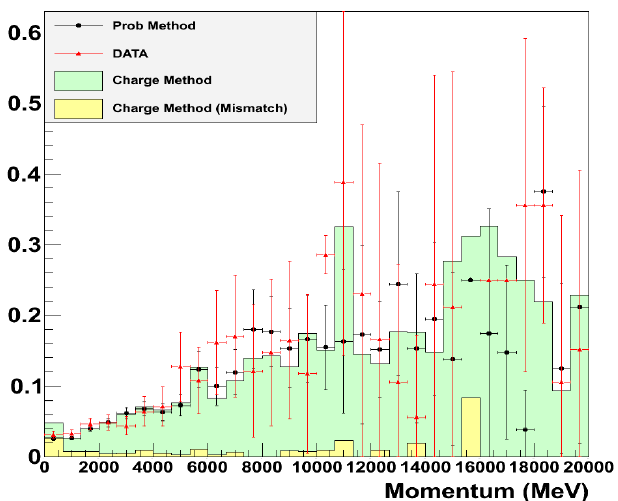
\includegraphics[width=5in]{Figures/Systematics/chmisID1.png}
\caption{The charge mis-ID rate vs. track momentum as calculated using the probability method (points) and charge method (fill)  \cite{chmisidtn}. All tracks used have a minimum of 18 nodes. The mis-ID rates in data (red) are calculated with the probability method.}
\label{fig:chmisid}
\end{figure}

The next step of the procedure is to propagate these charge mis-ID values to a systematic error on the data to MC ratio. The following observations concerning our selection significantly simplify the propagation of the charge mis-ID systematic:
\begin{enumerate}
\item The vast majority of selected muon tracks have $> 40$ nodes in the TPC constituent
\item The charge of the track is extracted only from TPC1, which makes the analysis insensitive to any mis-ID rates from TPC3 or any global charge reconstruction algorithms
\item As the tracks have a reconstructed vertex in the P0D, most are forward going.
\end{enumerate}

To propagate the charge mis-ID systematic into our analysis, we use a simple approach. We begin with samples extracted from the entire data and Monte Carlo sets by excluding the charge cut that is the very last CC inclusive cut. So we have quality matched tracks both positive and negative that originate in the P0D and pass through TPC1. This data and MC sample is further classified into two mutually exclusive subsets:

\begin{enumerate}
\item Beam bunches where the highest momentum track is reconstructed as positive
\item Beam bunches where the highest momentum track is reconstructed as negative
\end{enumerate}

If a track in subset 1 had been misreconstructed as positive when in truth it was negative, then it is a candidate muon track which we missed. To correct for this, we must add the number of charge misidentified tracks in subset 1 to the total number of selected CC inlcusive events. Similarly, if a track in subset 2 had been misreconstructed as negative when in truth it was positive, then we must remove it from the number of candidate CC inclusive events. To calculate the number of tracks in each subset that were reconstructed with incorrect charge, we simply multiply by the charge mis-ID rate. So the corrected number of events after adjusting for charge mis-ID is given by:

\begin{center}
$N^{corr}(i) = N(i)+P(i)\cdot\left(N^{1}(i)-N^{2}(i)\right)$.
\end{center}

$N(i)$ is total number of events in subset 2 in a particular momentum bin $i$ and $N^{corr}(i)$ is the charge mis-ID corrected value in the same momentum bin. We chose to use subset 2 for the value of $N(i)$ as it is almost identical to the CC inclusive selection. $P(i)$ represents the probability of charge mis-ID in momentum bin $i$ extracted directly from Ref \cite{chmisidtn} except for one small change. Negative probabilities are unphysical so we ignore them and set them to zero. Any error on the probability is change to match (ex:$-0.2\pm 1$ is changed to $0 + 0.8$). Finally, $N^1$ and $N^2$ are the total number of tracks in subsets 1 and 2 respectively. Table \ref{tab:N_posneg} summarizes the number of tracks in each subset for different momentum bins in both data and MC. Tables \ref{tab:N_corr_w} and \ref{tab:N_corr_a} then show the charge mis-ID corrected number of CC inclusive events for data and MC in water-in and water-out data respectively. 

\begin{table}
\caption{Number of data and MC events in subset 1 and 2 for both runs. MC values are normalized by POT, not flux-reweighted and not corrected for fiducial mass discrepancy.}
\label{tab:N_posneg}
\centering
\begin{tabular}{cccccc}\toprule
Data / MC & Mom. bin & Subset 1 & Subset 2 & Subset 1 & Subset 2\\
& Water-in & Water-in & Water-out & Water-out \\\midrule
& 0-1.3 GeV & 667 & 2463 & 1705 & 5627\\
& 1.3-2.6 GeV & 220 & 983 & 486 & 1995\\
Data & 2.6-4.0 GeV & 59 & 568 & 170 & 1290\\
& 4.0-5.3 GeV & 21 & 286 & 62 & 551\\
& 5.3+ GeV & 54 & 359 & 117 & 719 \\\midrule
& 0-1.3 GeV & 701 & 2672 & 1886 & 5959\\
& 1.3-2.6 GeV & 229 & 1025 & 547 & 2122\\
MC & 2.6-4.0 GeV & 90 & 689 & 222 & 1409\\
& 4.0-5.3 GeV & 34 & 350 & 83 & 731\\
& 5.3+ GeV & 56 & 404 & 122 & 891 \\
\bottomrule
\end{tabular}
\end{table}

\begin{table}
\caption{The charge mis-ID rate and the corrected number of CC inclusive events for data and MC in different momentum bins for water-in.}
\label{tab:N_corr_w}
\centering
\begin{tabular}{ccccc}\toprule
Mom. bin & Data Mis-ID Rate(\%) & MC Mis-ID Rate(\%) & $N^{corr}_{Data}$ & $N^{corr}_{MC}$ \\\midrule
0-1.3 GeV & $0+0.8$ & $0+0.1$ &2463.0 &2672.0 \\
1.3-2.6 GeV & $1.4\pm 0.7$ & $2.1\pm 0.1$  & 972.3 & 1008.5 \\
2.6-4.0 GeV & $3.3\pm 1.3$ & $4.5\pm 0.1$ & 551.2 & 661.8 \\
4.0-5.3 GeV & $6.1\pm 2.5$ & $4.5\pm 0.2$ & 269.8 & 335.9 \\
5.3+ GeV & $12\pm 3$ & $13.1\pm 0.2$  & 322.4 & 358.5 \\\midrule
Total & --  & --  & 4578.8 & 5036.7\\
\bottomrule
\end{tabular}
\end{table}

\begin{table}
\caption{The charge mis-ID rate and the corrected number of CC inclusive events for data and MC in different momentum bins for water-out.}
\label{tab:N_corr_a}
\centering
\begin{tabular}{ccccc}\toprule
Mom. bin & Data Mis-ID Rate(\%) & MC Mis-ID Rate(\%) & $N^{corr}_{Data}$ & $N^{corr}_{MC}$ \\\midrule
0-1.3 GeV & $0+0.8$ & $0+0.1$ & 5627.0 & 5958.7 \\
1.3-2.6 GeV & $1.4\pm 0.7$ & $2.1\pm 0.1$  & 1973.9 & 2089.1 \\
2.6-4.0 GeV & $3.3\pm 1.3$ & $4.5\pm 0.1$ & 1253.0 & 1355.7 \\
4.0-5.3 GeV & $6.1\pm 2.5$ & $4.5\pm 0.2$ & 521.2 & 701.7 \\
5.3+ GeV & $12\pm 3$ & $13.1\pm 0.2$  & 646.8 & 791.3 \\\midrule
Total & --  & --  &10021.8 & 10896.6\\
\bottomrule
\end{tabular}
\end{table}

To extract systematics from Tables \ref{tab:N_corr_w} and \ref{tab:N_corr_a}, we recalculate the data/MC ratio with the corrected values and take the difference from the nominal ratio. The nominal ratio is defined as the data/MC ratio from the total number of events in subset 2. %The nominal ratio is 98.23\% and the corrected ratio is 98.56\%, which yields a systematic difference of 0.33\%.
The errors on the charge mis-ID values are on the order of the misidentification rate itself, so we cannot ignore them. To be conservative, we linearly added and subtracted the mis-ID rate with the error in each bin. Any negative probabilities were set to 0. The change in data/MC ratio was calculated for both the cases where all the mis-ID rates had gone up by 1 $\sigma$ and gone down by 1 $\sigma$. The larger change is assigned as a symmetric systematic error. We find a systematic of $\pm 0.75\% $ and $\pm 0.72\%$ from the charge mis-ID rate for water-in and water-out running respectively.

\subsection{Summary of Detector Systematic Uncertainties}

We have evaluated detector systematic corrections and errors on the data to MC ratio from several sources. The effects of hit reconstruction efficiency, neutral back scattering, sand muon contamination, event pile-up, track timing and the cosmic background are all negligible and have not been assigned any systematic errors. Track matching efficiency and the sand muon interference rate both cause systematic shifts in the central value data to MC ratio. Therefore these two effects have a systematic correction as well as a systematic error associated with them. The corrections are applied in the next section while the errors are summarized here. All the non-negligible systematic errors on the data to MC ratio are summarized in Table \ref{tab:syssum}. These errors must still be propagated to the absolute cross section measurement. The process of calculating an error on the cross section from the values in Table \ref{tab:syssum} is discussed in the following section.

\begin{table}[h]
\caption{Summary of non-negligible fractional detector systematic uncertainties on the data to MC ratio of CC inclusive event rate for water-in and water-out samples.}
\label{tab:syssum}
\centering
\begin{tabular}{ccc}
\toprule
Systematic Source & Water-in & Water-out\\
\midrule
P0D Tracking and Matching Efficiency & $^{+0.00447}_{-0.00447}$ & $^{+0.00541}_{-0.00541}$\\[2pt]\midrule
Fiducial Volume & $^{+0.00301}_{-0.00727}$ & $^{+0.00262}_{-0.00024}$\\[2pt]\midrule
Sand Interference & $^{+0.01190}_{-0.01160}$ & $^{+0.01380}_{-0.01440}$\\[2pt]\midrule
Out of Fiducial Volume & $^{+0.00027}_{-0.00027}$ & $^{+0.00262}_{-0.00024}$\\[2pt]\midrule
TPC1 Tracking Efficiency & $^{+0.00164}_{-0.00164}$ & $^{+0.00135}_{-0.00135}$\\[2pt]\midrule
Charge Mis-ID & $^{+0.00685}_{-0.00685}$ & $^{+0.00649}_{-0.00649}$\\[2pt]
\bottomrule
\end{tabular}
\end{table}

\clearpage

\section{Detector Systematic Corrections and Uncertainties}
\label{sec:detsysprop}

In the previous Section we evaluated the detector systematic corrections and uncertainties on the data/MC ratio. In this Section, we first take the systematic corrections and apply them to the central value of the water cross section. Then we propagate the data/MC errors to and error range on the cross section measurement. All of the work in this Section is specific to our analysis and therefore completed by us.

\subsection{Detector Systematic Corrections}

During the evaluation of the systematic uncertainties on the data/MC ratio, we found several inaccuracies that require a correction to the central value of the cross section measurement. There are three major corrections that are applied: fiducial mass, matching efficiency and sand muon interference. The fiducial mass in the MC is slightly different than the surveyed mass of the actual detector as shown in Table \ref{tab:fidmass}. There is also a minor difference between MC and data in the expected matching efficiency when pairing together tracks from the P0D and Tracker reconstruction algorithms. The matching efficiency systematic from Section \ref{sec:matchingsyst} yields a small correction to the absolute water cross section. Finally, as discussed in Section \ref{sec:sandintsys}, we expect that there is a difference in the reconstruction failure rate in data and MC caused by external sand muon tracks. These tracks are concurrent in time with candidate CC inclusive muon tracks. As the sand muon rate is not very well known, and as this rate also depends on the beam intensity, we apply a run by run correction to the MC event rate before extracting the absolute water cross section. 

To apply these corrections, we rewrite the water subtraction formula in equation \ref{eqn:xsec6} as follows:
\begin{equation}
\sigma_w = \frac{1}{T_w}\left[\frac{1}{\sum\limits_r \Phi_1(r)}\sum\limits_{r}^{1,2,4} \sum\limits_{z}^{40} \frac{N^{obs}_1(r,z)-B^{pred}_1(r,z)}{\epsilon^{pred}_1(r,z)}-\frac{1}{\sum\limits_r \Phi_2(r)}\sum\limits_{r}^{2,3,4} \sum\limits_{z}^{40} \frac{N^{obs}_2(r,z)-B^{pred}_2(r,z)}{\epsilon^{pred}_2(r,z)}\right].
\end{equation}
Here the $B^{pred}$ and $\epsilon^{pred}$ terms are corrected from the nominal MC prediction. How these terms are corrected is described below.

\begin{table}[h]
\caption{The mass in the P0D fiducial volume for water-in and water-out run periods.}
\label{tab:fidmass}
\centering
\begin{tabular}{cccc}\toprule
Mass (kg) & Water-in & Water-out & Water-only \\\midrule
As-built (run 1) & $5460.86 \pm 37.78$ & $3558.86 \pm 34.23$ & $1902 \pm 16$\\
As-built (run 2)& $5480.30 \pm 37.40$ & $3578.30 \pm 33.80$ & $1902 \pm 16$\\
MC Prod. 5 & $5393.22\pm 0.56$ & $3469.14 \pm 0.55$ & $1927.5 \pm 0$ \\
\bottomrule
\end{tabular}
\end{table}

The fiducial mass correction changes only one term in the cross section formula, specifically, the MC predicted background. The adjusted background term is:
\begin{equation}
B^{pred} = C^{FM} * B^{MC}.
\end{equation}
The $C^{FM}$ term is the ratio of as-built fiducial mass to the MC fiducial mass calculated from Table \ref{tab:fidmass}. For run 1, the correction used is the ratio of the nominal fiducial mass values in row 3 and row 1. For all other runs, the correction is the ratio of row 3 and row 2. Corrections for water-in and water-out run periods are calculated separately using the water-in and water-out columns of Table~\ref{tab:fidmass}. As the number of neutrino interactions is directly proportional to the amount of target material, the $C^{FM}$ term corrects the MC background to what we would expect in the data given the slightly different fiducial mass. We do not apply any correction to the efficiency term as both the numerator and denominator of the efficiency scale the same way with a change in fiducial mass. 

The cosmics matching efficiency study yielded a data matching efficiency of $99.08\% \pm 0.16\%$ and MC matching efficiency of $99.22\% \pm 0.24\%$. We calculate that the multiplicative shift in the data/MC ratio from this small difference in matching efficiency is equal to the MC matching efficiency divided by the data matching efficiency. This yields a correction factor of $1.0014 \pm 0.0024\%$. The hand scanning study yielded a difference in the rate of anomalous matching failures between data and MC. The data was found to have more failures than the MC. To correct for this difference, we calculated that the data/MC ratio should be multiplied by $1.017 \pm 0.0039$ for water-in and by $1.023 \pm 0.0053$ for water-out. The data/MC ratio shifts from the cosmics study and hand scan study are combined multiplicatively and the errors added in quadrature. This yields a total data/MC ratio shift of $1.018 \pm 0.0049$ for water-in and $1.024 \pm 0.0060$ for water-out.

The matching efficiency correction applied in this analysis is equal to the central value of the shift in the data/MC ratio. The error in this shift is treated later as a systematic error. The matching efficiency correction affects two terms in the cross section formula: the background and the efficiency. Similar to the fiducial mass correction, the MC background is multiplied by the matching efficiency correction term to properly predict the amount of background expected in the data. As the matching efficiency only affects the process of selection and not the total number of signal interactions generated, we multiply the numerator of the signal efficiency term by the correction factor. So the signal efficiency term now looks like

\begin{equation}
\epsilon^{pred} = C^{eff.}* \epsilon^{MC}.
\end{equation}

The sand muon correction is also applied to our absolute water cross section measurement. The sand muon veto procedure yields a discrepancy in the number of events vetoed between data and MC. As sand muon interactions are simulated separately from the beam MC, there are no potential events in the MC selection that have both a sand muon track and a true CC inclusive track concurrent in time. This difference is corrected with a small multiplicative factor to the total MC events selected. To find this multiplicative factor, we compare the veto survival rates ($R_{veto}$) in data and MC. Here $R_{veto}$ is equal to the number of selected events after the sand muon veto divided by the number of selected events before the sand muon veto. The difference in data and MC veto survival rate is used to calculate the correction factor ($C^{SM}$) due to sand muon interference,

\begin{equation}
C^{SM} = 1-(R^{MC}_{veto} - R^{Data}_{veto})
\end{equation}

\noindent where $R^{MC}_{veto}$ and $R^{Data}_{veto}$ are the sand muon veto survival ratios for data and MC respectively. Also note that since the beam power changes for every run and run type, $C^{SM}$ is actually a function of run (i.e. $C^{SM} \rightarrow C^{SM}(r)$). Although sand muons are technically a source of background, in this case the sand muon interference causes us to potentially veto perfectly good signal events. This affects both the calculated efficiency and the MC predicted background. The sand muon interference correction factor is therefore applied both to the background and signal efficiency terms in our cross section equation. Table \ref{tab:smcorr} lists the values for $C^{SM}$ calculated from Table \ref{tab:rveto}. 

\begin{table}[h]
\caption{The sand muon interference correction $C^{SM}$ for each run number and run type.}
\label{tab:smcorr}
\centering
\begin{tabular}{cc}\toprule
Run \#/type & $C^{SM}$ \\ \midrule
Run 1 water-in & 0.9934 \\
Run 2 water-in & 0.9954 \\
Run 2 water-out & 0.9811 \\
Run 3 water-out & 0.9924 \\
Run 4 water-in & 0.9894 \\
Run 4 water-out &  0.9830 \\
\bottomrule
\end{tabular}
\end{table}

Putting the three corrections together, the cross section formula is now:

\begin{multline}
\label{eqn:nomxsec}
\sigma_w = \frac{1}{T_w} \left[ \frac{1}{\sum\limits_r \Phi_w(r)}\sum\limits_{r}^{1,2,4} \sum\limits_{z}^{40} \frac{N^{obs}_w(r,z)-(C_w^{FM}*C_w^{eff}*C_w^{SM}(r))B^{MC}_w(r,z)}{C_w^{eff}*C_w^{SM}(r)*\epsilon^{MC}_w(r,z)} \right. \\
	\left. -\frac{1}{\sum\limits_r \Phi_a(r)}\sum\limits_{r}^{2,3,4} \sum\limits_{z}^{40} \frac{N^{obs}_w(r,z)-(C_a^{FM}*C_a^{eff}*C_a^{SM}(r))B^{MC}_w(r,z)}{C_a^{eff}*C_a^{SM}(r)*\epsilon^{MC}_w(r,z)}\right].
\end{multline}

Using the correction factors described above, the new central value for the absolute water cross section is
\begin{equation}
\left<\sigma\right>_\Phi = 6.37\times 10^{-39} \frac{\text{cm}^2}{H_2O\:\text{nucelon}}.
\end{equation}
This can be compared to the uncorrected cross section value of $6.51\times 10^{-39}$ cm$^2$/nucleon.

\subsection{Detector Systematic Uncertainties}

In previous sections, we evaluated the systematic uncertainty on the data/MC ratio of CC inclusive events rates. In this section, we discuss the propagation of these detector systematic errors. There are seven sources of detector systematic uncertainty that are calculated. To propagate them to the absolute water cross section measurement, we use a very simple and straightforward approach. Each of the seven systematics yield a small error on the MC background, the MC efficiency or both. So for each systematic source, we evaluate the fractional variation on the absolute water cross section $(\delta\sigma)$ using the following familiar formula:

\begin{multline}
\label{eqn:finalxsec}
\sigma_w = \frac{T_w}{\sigma_{nom}}\left[\frac{1}{\sum\limits_r \Phi_w(r)}\sum\limits_{r}^{1,2,4} \sum\limits_{z}^{40} \frac{N^{obs}_w(r,z)-(f_w^{BG sys.})B^{MC}_w(r,z)}{f_w^{eff. sys.}*\epsilon^{MC}_w(r,z)}
\right. \\
\left. -\frac{1}{\sum\limits_r \Phi_a(r)}\sum\limits_{r}^{2,3,4} \sum\limits_{z}^{40} \frac{N^{obs}_w(r,z)-(f_a^{BG sys.})B^{MC}_w(r,z)}{f_a^{eff. sys.}*\epsilon^{MC}_w(r,z)}\right].
\end{multline}

Here, $\sigma_{nom}$ is the nominal cross section calculated in the previous subsection. The factors in front of the background and efficiency come directly from Table \ref{tab:syssum}. They are scale factors that allow us to vary the background and efficiency by 1$\sigma$ excursions for any given systematic. The scale factors are calculated very simply.

When a detector systematic is varied, the ratio of the number of selected CC inclusive events in data (D) to the number in MC (M) also varies. The fractional variation from the nominal ratio ($R = D / M$) to the new ratio ($R' = D' / M'$), is what is used as a systematic error in Ref\cite{tn80}. Here, we use the same fractional variation $\delta R = \frac{R' - R}{R}$ to calculate the scale factors. By assuming that the number of selected CC inclusive events in data remains the same when varying a detector systematic, we assert that the entirety of the data to MC ratio difference must be due to a change in the MC event rate(i.e. $M^{old} \rightarrow M^{new}$). As the scale factors ($f^{sys}$) for background and signal efficiency should be ($M^{new} / M^{old}$), we calculate that they are related to $\delta R$ as follows:

 %by using the fractional systematic error on the data/MC ratio. For example, for a systematic with a fractional error of $\delta r$ of the data to MC ratio, the scale factor on the water background term would be:

\begin{equation}
 f^{BG sys.}_w =  \frac{1}{1+\delta R}.
\end{equation}

Note that this actually is a very conservative approach as we assume the MC predictions of background and signal efficiency are as different from the data as our measurements allow. The fractional systematic errors in the data/MC ratio are taken directly from Table \ref{tab:syssum}. Instead of using different upward and downward fluctuations in the fractional errors, for each detector systematic, we assign the larger variation as a symmetrical fractional error. Finally, we evaluate $\delta\sigma$ for both the upward and the downward fluctuation of the detector systematic and once again take the larger variation as the symmetric fractional systematic uncertainty on the absolute water cross section.

There are two more considerations before calculating the detector systematic uncertainty in this fashion. First, just like the fiducial mass and matching efficiency corrections, not all systematics sources affect both the background and signal efficiency predictions. For each systematic, we must decide whether to vary both the background and the signal efficiency or just one of the two. In such cases, the unaffected scale factors $f$ are set to 1. Second, we must consider whether or not the uncertainty is correlated between water-in running and water-out running. As we do not directly calculate the correlation coefficient, we estimate them by choosing a correlation coefficient value of 1, 0 or -1 (i.e. fully correlated, uncorrelated and anticorrelated). This decision is made logically by examining whether the source of an error remains unchanged between water-in and water-out running. We find that only one error source is uncorrelated while the rest are fully correlated. There are no errors that are assumed anticorrelated. The specifics for each error source are discussed below. 

In the case of correlated errors, we calculate $\delta\sigma$ by making $1\sigma$ variations simultaneously in the water-in and water-out terms of the cross section formula (i.e. $f_w^{BG sys.}$, $f_w^{eff. sys.}$, $f_a^{BG sys.}$ and $f_a^{eff. sys.}$ are all set to their respective 1$\sigma$ values). In this case, we calculate $\delta\sigma$ twice, once for a 1$\sigma$ variation in just the water-in scale factors (i.e.  $f_w^{BG sys.}$ and $f_w^{eff. sys.}$ are set to 1$\sigma$ variation values while $f_a^{BG sys.}$ and $f_a^{eff. sys.}$ are set to 1) and once for a 1$\sigma$ variation in just the water-out terms. The two $\delta r$'s are added in quadrature to yield the systematic uncertainty on the absolute water cross section for that source.

The list of significant detector systematics, a brief comment on water-in/water-out correlation and the effect on predicted background/signal-efficiency are provided below.
\begin{itemize}
\item P0D Tracking and Matching Efficiency: The track reconstruction software uses hits generated by particles passing through scintillator bars in the P0D. The matching algorithm then pairs together reconstructed tracks from the P0D and Tracker. Neither of these pieces of code depends on the presence of water in the P0D as there are no additional hits generated in the water. The water-in and water-out running periods then have fully correlated tracking/matching uncertainties. As argued in the previous subsection, the matching efficiency affects both the predicted background and the signal efficiency.
\item Fiducial Mass: The total fiducial mass error is calculated from two sources: the P0D material fiducial mass and the water fiducial mass. The water-out P0D material uncertainty is fully correlated between water-in and water-out running. As the mass of the water-out P0D does not change, this systematic error is neglected. The water fiducial mass uncertainty is only applied to the water-in terms. From Table \ref{tab:fidmass}, we find that the fractional uncertainty on water-only is 16/1902 = 0.84\%. As argued in the previous subsection, the fiducial mass variation does not affect the signal efficiency prediction. However, this is the only detector systematic that results in a variation in the total nucleons in water, $T_w$, used in Formula \ref{eqn:finalxsec}.
\item Fiducial Volume: This error accounts for any large potential differences in vertex distributions in the P0D at the edges of the fiducial volume cut. The fiducial volume systematic section describes this effect in greater detail. The distributions are known to be smooth and the individual systematic is small. The positioning of the vertex relies on the available hits in the P0D and not on the presence of water in the bags although there is an energy loss dependence. As such, the shape of the vertex distributions are arguably unrelated to whether the P0D is in water-in or water-out running mode. The error is treated as fully correlated. This is a selection cut and therefore affects the background prediction as well as the selected signal efficiency.
\item Out-of-Fiducial-Volume: We do not have sufficient information to argue correlation between water-in and water-out. The amount of background certainly varies as a function of the amount of mass in the P0D. We do however believe that there is no reason this error is anticorrelated. Therefore, we take the conservative approach and treat this error as uncorrelated, yielding the largest error. Again, as this is a background source, we only vary the background prediction scale factors for this.
\item Sand Muon Contamination: The sand muon simulation is somewhat different from what the data observes. We calculate an error to account for the possible excess of sand muons observed in data even though our veto power is excellent. The generation of sand muons is unrelated to the presence of water in the P0D and so the systematic is treated as fully correlated between water-in and water-out. Although sand muons are actually background, its primary effect in our analysis is to cause false-vetos of genuine CC inclusive events. In this way, the sand muon contamination changes the signal selection itself. Therefore both the background and signal efficiency scale factors are varied for this systematic.
\item TPC1 tracking efficiency: This is a detector systematics that has no dependence on water as the Tracker remains the same through all run periods. This error is fully correlated. Also, a track must be found from the Tracker to pass the selection so both background and signal efficiency scale factors are affected.
\item Charge Mis-ID: Similar to the TPC1 tracking efficiency, the charge mis-id error rate has no dependence on water in the P0D. This error is also fully correlated. Also, the charge measurements from the Tracker are used in the selection so both background and signal efficiency scale factors are affected.

\end{itemize}

We then use the argued detector systematic correlations and the data to MC ratio systematic values to calculate the fractional systematic uncertainty on the absolute water cross section measurement for each source. The systematic sources are estimated to be uncorrelated to each other. So we add the errors in quadrature to evaluate the total uncertainty. The results are summarized in Table \ref{tab:detsys}. The fractional systematic errors from Table \ref{tab:syssum} are summarized in columns 2 and 3 for water-in and water-out. The resulting fractional error in the absolute water cross section is shown in column 4.

\begin{table}[h]
\caption{Summary of Detector Systematic Errors for runs 1-4 and the resulting fractional error on the absolute water cross section.}
\centering
\begin{tabular}{lccc}\toprule\midrule
\renewcommand{\arraystretch}{1.1}
Systematic Source & Water-in $\delta r$  & Water-out $\delta r$ & $\delta\sigma$ frac.
\\ \midrule
P0D Tracking and Matching Efficiency & 0.0047 & 0.00541 & 0.0033\\
\midrule
Fiducial Mass & 0.0084 & 0 & 0.0064\\
\midrule
Fiducial Volume & 0.00727 & 0.00262 & 0.0156\\
\midrule
Out of P0D FV & 0.00027 & 0.00054 & 0.0001\\
\midrule
Sand Muon BG & 0.0119 & 0.0138 & 0.0072\\
\midrule
TPC1 Tracking Efficiency & 0.00164 & 0.00135 & 0.0021\\
\midrule
Charge Mis-ID & 0.00685  & 0.00649 & 0.0074\\
\midrule
\midrule
Total Det. Sys. &  - & - & 0.0202  \\
\midrule
\bottomrule
\end{tabular}
\label{tab:detsys}
\end{table}

The total fractional detector systematic uncertainty on the absolute water cross section is $2.02\%$. As expected, it is the smallest uncertainty when compared to flux and cross section model systematics. The small size of the detector systematic is possible due to the subtraction measurement as the correlations between water-in and water-out allow us to reduce overall error.

\subsection{Statistical Uncertainty}

We assume Poissonian errors on the event rates in each bin and propagate the cross section error following basic error analysis formulae. As we are only concerned with the statistical error from the number of selected events in data, we treat the target number, integrated flux terms, efficiency terms, background terms and correction factors as constants. Then Equation~\ref{eqn:nomxsecerr} yields the statistical variance on the cross section measurement and comes directly from the formula in Equation~\ref{eqn:nomxsec} for the nominal cross section:

\begin{multline}
\label{eqn:nomxsecerr}
\delta(\sigma_w)^2 = \frac{1}{T_w^2} \left[ \frac{1}{\left(\sum\limits_r \Phi_w(r)\right)^2} \sum\limits_{r}^{1,2,4} \sum\limits_{z}^{40} \frac{N^{obs}_w(r,z)}{(C_w^{eff}*C_w^{SM}(r)*\epsilon^{MC}_w(r,z))^2} \right. \\
	\left. +\frac{1}{\left(\sum\limits_r \Phi_a(r) \right)^2}\sum\limits_{r}^{2,3,4} \sum\limits_{z}^{40} \frac{N^{obs}_w(r,z)}{(C_a^{eff}*C_a^{SM}(r)*\epsilon^{MC}_w(r,z))^2}\right].
\end{multline}
We find an absolute statistical error of $1.57\times 10^{-40}$ which is 2.47\% fractionally on the cross section measurement.

